\documentclass[11pt]{article}

% ---- Packages ----
\usepackage[utf8]{inputenc}
\usepackage[T1]{fontenc}
\usepackage{amsmath,amssymb,amsfonts}
\usepackage{graphicx}
\usepackage{booktabs}
\usepackage{hyperref}
\usepackage{url}
\usepackage{xcolor}
\usepackage{subcaption}
\usepackage[margin=1in]{geometry}
\usepackage{natbib}
\usepackage{microtype}
\usepackage{float}

% ---- Commands ----
\newcommand{\jaxcc}{\textsc{JAX-CrossCat}}
\newcommand{\crosscat}{\textsc{CrossCat}}
\newcommand{\jax}{\textsc{JAX}}
\newcommand{\xla}{\textsc{XLA}}

% ---- Title ----
\title{\jaxcc{}: GPU-Accelerated Bayesian Nonparametric\\Cross-Categorization in JAX}

\author{
  Pingal Singh \\
  Sambhal Labs \\
  \texttt{contact@sambhal-labs.com}
}

\date{}

\begin{document}
\maketitle

% ============================================================================
\begin{abstract}
We present \jaxcc{}, a GPU-accelerated reimplementation of CrossCat
\citep{mansinghka2016crosscat} in JAX. The original Python~2/C++
implementation is unmaintained and cannot exploit GPUs. \jaxcc{} achieves
up to $619\times$ aggregate kernel-level speedup on a P100 GPU through
six innovations: (1)~a fixed-size packed state for JIT compilation,
(2)~unified type dispatch eliminating Python branching across five column
types, (3)~\texttt{vmap}/\texttt{lax.scan} vectorization of all Gibbs
kernels, (4)~type-specialized fast paths for homogeneous views,
(5)~batched sufficient statistic updates via matrix operations, and
(6)~multi-GPU chain distribution via \texttt{jax.pmap}, achieving
$3.3\times$ throughput scaling on $2\times$~T4 GPUs. We
reproduce key experiments from the original paper --- MNIST
classification (89\% multi-chain, 93.6\% inpainting at 30\% observation)
and synthetic structure recovery (ARI~$= 1.0$) --- and present new
results on macroeconomic data (217~countries $\times$ 95~indicators) and
scalability up to $2{,}000 \times 2{,}000$ tables. The library comprises
${\sim}$12,500 lines of Python, validated by 333~tests including
34~Hypothesis property tests, and is source-available under the Business
Source License~1.1.
\end{abstract}

% ============================================================================
\section{Introduction}
\label{sec:intro}

High-dimensional datasets containing variables of heterogeneous types
are ubiquitous in science, medicine, economics, and industry. Analyzing
such data requires methods that can simultaneously model continuous,
categorical, binary, ordinal, and cyclic variables; detect dependencies
and independencies between variables; handle missing data; and quantify
uncertainty in predictions. CrossCat \citep{mansinghka2016crosscat} is a
fully Bayesian nonparametric method that addresses these challenges by
positing a hierarchical Dirichlet process mixture model: an outer DP
partitions columns into independent \emph{views}, and an inner DP per
view clusters rows into \emph{categories}. All continuous parameters are
collapsed out via conjugate Bayesian component models, leaving only
discrete cluster assignments and hyperparameters to be sampled via Gibbs
MCMC.

Despite its theoretical elegance and strong empirical results on datasets
of up to 10~million cells, the original CrossCat implementation
\citep{mansinghka2016crosscat} faces three practical barriers to
adoption. First, it is written in Python~2 with ${\sim}$4,000 lines
of C++ and is no longer maintained. Second, it cannot exploit modern GPU
hardware --- its Gibbs sampler uses sequential Python loops over rows,
columns, views, and clusters. Third, extending the system with new
column types or inference queries requires modifying both the Python and
C++ codebases.

We present \jaxcc{}, a complete reimplementation in JAX
\citep{jax2018github} that overcomes these barriers. Our key
contributions are:

\begin{enumerate}
  \item A \textbf{packed state representation} that encodes the variable-size
    CrossCat state as fixed-size JAX arrays, enabling JIT compilation of
    the entire Gibbs sampler.
  \item \textbf{Unified type dispatch} via \texttt{jnp.where} that
    evaluates all five column types simultaneously without Python
    branching, plus type-specialized fast paths for homogeneous views.
  \item \textbf{Vectorized Gibbs kernels} using \texttt{jax.vmap} for
    parallel scoring across columns, clusters, and rows, and
    \texttt{jax.lax.scan} for sequential sweeps --- yielding a single
    compiled GPU kernel per sweep.
  \item \textbf{Batched sufficient statistics} via matrix operations
    (scatter-add, einsum) that replace nested Python loops for
    incremental updates.
  \item A comprehensive \textbf{inference query library} with 29
    vectorized posterior predictive functions, multi-chain aggregation,
    online row insertion, and dependency constraints.
  \item \textbf{Multi-GPU inference} via \texttt{jax.pmap} and
    \textbf{scaling utilities} (subsample initialization, mini-batch
    Gibbs sweeps, early stopping) for datasets with 10K+ rows.
\end{enumerate}

\jaxcc{} reproduces the experimental results from
\citet{mansinghka2016crosscat} and extends them with new benchmarks on
macroeconomic data, multi-GPU throughput, and scalability measurements up
to $2{,}000 \times 2{,}000$ tables. The library is
source-available\footnote{\url{https://github.com/sambhal-labs/jaxcross}
--- Business Source License~1.1; free for non-production use, converts to
Apache~2.0 after four years.} and installable via \texttt{pip}.

% ============================================================================
\section{Background}
\label{sec:background}

\subsection{The CrossCat Model}

CrossCat \citep{mansinghka2016crosscat} is a Bayesian nonparametric
model for tabular data $\mathbf{X} \in \mathbb{R}^{R \times D}$, where
$R$ is the number of rows (entities) and $D$ the number of columns
(variables). The generative process unfolds in three stages:

\begin{enumerate}
  \item \textbf{Column partitioning.} A concentration parameter
    $\alpha_D$ is drawn from a Gamma prior. Each column $d$ is assigned
    to a view $z_d$ via a Chinese Restaurant Process (CRP) with
    concentration $\alpha_D$:
    \begin{equation}
      \alpha_D \sim \mathrm{Gamma}(1, 1), \qquad
      z_d \sim \mathrm{CRP}(\{z_i \mid i \neq d\}; \alpha_D).
    \end{equation}

  \item \textbf{Row clustering per view.} For each view $v$, a
    concentration parameter $\alpha_v$ is drawn, and rows are assigned to
    categories via an inner CRP:
    \begin{equation}
      \alpha_v \sim \mathrm{Gamma}(1, 1), \qquad
      y_r^v \sim \mathrm{CRP}(\{y_i^v \mid i \neq r\}; \alpha_v).
    \end{equation}

  \item \textbf{Data generation.} For each cluster $c$ in the row
    partition $\vec{y}^v$ of view $v$, and each column $d$ assigned to
    that view, data is generated from a type-specific component model
    with hyperparameters $\vec{\lambda}_d$ drawn from a vague prior
    $V_d$:
    \begin{equation}
      \vec{x}^c_{(\cdot,d)} \sim ML_d(T_d(\vec{x}^c_{(\cdot,d)}); \vec{\lambda}_d),
    \end{equation}
    where $ML_d$ is the marginal likelihood under conjugate
    prior--likelihood pairs and $T_d$ extracts sufficient statistics.
\end{enumerate}

\subsection{Component Models}

\jaxcc{} supports five column types with conjugate (or approximately
conjugate) component models:

\begin{itemize}
  \item \textbf{Continuous} --- Normal-Gamma: $(\mu, \sigma^2) \sim
    \mathrm{NormalGamma}(\mu_0, \kappa, \nu, s)$, likelihood
    $\mathcal{N}(\mu, \sigma^2)$. Posterior predictive is Student-$t$.
  \item \textbf{Categorical} --- Dirichlet-Multinomial: symmetric
    Dirichlet prior with concentration $\alpha$, multinomial likelihood.
  \item \textbf{Binary} --- Beta-Bernoulli: $\theta \sim
    \mathrm{Beta}(\alpha, \beta)$, likelihood $\mathrm{Bernoulli}(\theta)$.
  \item \textbf{Ordinal} --- Ordered Logistic: non-conjugate; uses grid
    integration over a latent location parameter $\mu$ with fixed
    cutpoints.
  \item \textbf{Cyclic} --- Von Mises: directional data on $[0, 2\pi)$
    with conjugate updates for the mean direction and concentration.
\end{itemize}

The ordinal and cyclic types are new additions not present in the
original CrossCat, extending applicability to Likert-scale survey data
and angular measurements.

\subsection{Inference Algorithm}

Posterior inference follows the collapsed Gibbs sampling scheme from
\citet{mansinghka2016crosscat}, cycling through five kernels per sweep:

\begin{enumerate}
  \item \textbf{CRP concentration parameters}: Grid-based discrete
    approximation to the posterior for $\alpha_D$ and each $\alpha_v$.
  \item \textbf{Column hyperparameters}: Per-column, per-hyperparameter
    grid-based sampling from the approximate posterior.
  \item \textbf{Row assignments}: For each row in each view, sample a
    new cluster from the CRP-weighted posterior predictive likelihood
    across all existing clusters plus a new-cluster proposal (Algorithm~8
    of \citet{neal2000markov} with $m=1$).
  \item \textbf{Column assignments}: For each column, sample a new view
    assignment weighted by the marginal likelihood of the column's data
    under each view's clustering.
  \item \textbf{Cluster compaction}: Remove empty clusters and renumber
    to maintain contiguous indices.
\end{enumerate}

The original implementation executes these kernels via nested Python
for-loops with C++ inner loops. \jaxcc{} replaces this with a fully
JIT-compiled GPU pipeline, as described in Section~\ref{sec:system}.

% ============================================================================
\section{System Design}
\label{sec:system}

The central challenge in GPU-accelerating CrossCat is that the model
state has \emph{variable structure}: the number of views, clusters per
view, and columns per view all change during inference. JAX's JIT
compiler requires fixed array shapes. We address this through a
\emph{packed state representation} that encodes all variable-size
structures as fixed-size padded arrays.

\subsection{Packed State Representation}

The \texttt{PackedCrossCatState} dataclass contains 28 dynamic array
fields and 6 static shape parameters. Key design decisions:

\begin{itemize}
  \item \textbf{Pre-allocated capacity}: Arrays are padded to
    configurable maxima (\texttt{max\_views}, \texttt{max\_clusters},
    \texttt{max\_cols\_per\_view}). Active elements are tracked via
    count fields; inactive slots contain sentinel values.
  \item \textbf{JAX pytree registration}: The state is registered as a
    JAX pytree with array fields as dynamic children and shape parameters
    as static auxiliary data. This enables \texttt{vmap} and \texttt{jit}
    over states.
  \item \textbf{Bidirectional conversion}: \texttt{pack\_state()} converts
    the human-readable \texttt{CrossCatState} (Python lists of views) to
    the packed representation; \texttt{unpack\_state()} reverses it for
    inspection and inference queries.
  \item \textbf{Multi-chain batching}: \texttt{batch\_packed\_states()}
    stacks $N$ chains along a leading axis, enabling single-kernel
    multi-chain inference.
\end{itemize}

\subsection{Unified Type Dispatch}

CrossCat must evaluate component model scores for columns of different
types within the same view. Python implementations use \texttt{if/elif}
branches; this is incompatible with JIT compilation. We use
\emph{compute-all-select-one} dispatch:

\begin{equation}
  \mathrm{score}(x, \mathrm{type}_d) = \sum_{t=1}^{5}
  \mathbb{1}[\mathrm{type}_d = t] \cdot f_t(x, \vec{\lambda}_d, T_d),
\end{equation}

where $f_t$ is the scoring function for type $t$. While mathematically
only one term is nonzero, JAX's JIT compiler evaluates all five $f_t$
simultaneously --- the nested \texttt{jnp.where} implementation selects
the correct result after all branches execute. The compiler can sometimes
eliminate provably dead branches for statically-known types.

\paragraph{Type-specialized fast paths.} When all columns in a view
share the same type (e.g., all binary pixels in MNIST), the 5-way
dispatch is unnecessary. We detect this at the start of each row sweep
via \texttt{\_compute\_dominant\_type()} and route to batch-vectorized
type-specific scorers (e.g., \texttt{batch\_bb\_posterior\_predictive\_logp}
for binary). This optimization yielded a $12\times$ speedup for the
MNIST benchmark where 256 of 257 columns are binary.

\subsection{Vectorized Gibbs Kernels}

Each Gibbs kernel is rewritten to eliminate Python loops:

\begin{itemize}
  \item \textbf{Row scoring}: For a given row and cluster,
    \texttt{jax.vmap} computes the posterior predictive log-probability
    simultaneously across all columns in the view. A second \texttt{vmap}
    parallelizes across all candidate clusters.
  \item \textbf{Row sweep}: \texttt{jax.lax.scan} iterates over rows
    within a view (sequential, since each row's reassignment modifies the
    sufficient statistics for subsequent rows). An outer \texttt{lax.scan}
    iterates over views.
  \item \textbf{Column sweep}: \texttt{vmap} over columns, with an inner
    \texttt{lax.scan} over candidate views for each column.
  \item \textbf{Hyperparameter sweep}: \texttt{vmap} over columns,
    evaluating data-driven grids of 31 candidate values per
    hyperparameter.
\end{itemize}

Two sweep modes are provided: \texttt{packed\_gibbs\_sweep} wraps all
kernels in a single \texttt{lax.scan} over sweeps for maximum throughput;
\texttt{packed\_gibbs\_step} calls individually JIT-compiled sub-kernels
for interactive use and constraint enforcement.

\paragraph{Multi-chain and multi-GPU execution.}
\texttt{multi\_chain\_packed\_gibbs\_sweep} uses \texttt{jax.vmap} to
run $N$ chains as a single batched kernel call on one device. For
multi-GPU setups, \texttt{jax.pmap} distributes chains across devices
--- each GPU runs a subset of chains via \texttt{packed\_gibbs\_sweep}
internally. The MNIST benchmark (Section~\ref{sec:mnist}) uses this to
run 8~chains across $2\times$~T4 GPUs (4~per device). In the scalability
benchmark (Section~\ref{sec:scalability}), pmap achieves a $3.3\times$
throughput improvement for 4~chains on 2~devices compared to sequential
execution.

\subsection{Batched Sufficient Statistics}

Sufficient statistics are maintained as dense tensors of shape
$(V, K, C)$ where $V$, $K$, $C$ are \texttt{max\_views},
\texttt{max\_clusters}, and \texttt{max\_cols\_per\_view} respectively.
Recomputation from scratch uses membership-matrix multiplication:

\begin{equation}
  \mathbf{S}_{c,j} = \sum_{r=1}^{R} \mathbb{1}[y_r^v = c] \cdot x_{r,j},
\end{equation}

implemented via \texttt{jnp.einsum}. Incremental updates during row
reassignment use JAX's indexed scatter (\texttt{.at[].add()}) over all
columns simultaneously, replacing the original per-column Python loop.

\subsection{XLA Compilation Caching}

The first JIT compilation of \texttt{packed\_gibbs\_sweep} takes
${\sim}$22~seconds on a T4 GPU for typical problem sizes
($200 \times 10$), growing to ${\sim}$90~seconds for large problems
($2{,}000 \times 2{,}000$). We mitigate this via persistent XLA
compilation caching, automatically enabled on import. Compiled kernels
are stored to disk keyed on the static shape parameters. Subsequent
runs with the same shapes load cached executables, reducing startup
to ${<}\,1$~second.

\subsection{Inference Query Library}

Beyond MCMC sampling, \jaxcc{} provides 29 vectorized inference queries
on the packed state, all JIT-compiled:

\begin{itemize}
  \item \textbf{Predictive}: probability, sampling, CDF, credible
    intervals, joint probability
  \item \textbf{Anomaly detection}: per-row anomaly scores via posterior
    predictive log-probability
  \item \textbf{Imputation}: point estimates with confidence via
    posterior predictive mean/mode
  \item \textbf{Dependence}: pairwise dependence probability (Z-matrix),
    dependence matrix, mutual information
  \item \textbf{Similarity}: context-sensitive row similarity,
    row/column typicality
  \item \textbf{Online learning}: \texttt{packed\_insert\_rows} for
    streaming data without re-running full inference
\end{itemize}

Multi-chain wrappers aggregate results across independent chains via
posterior averaging.

\subsection{Scaling Utilities}

For datasets beyond ${\sim}$2,000 rows, the full row sweep becomes the
bottleneck ($O(R)$ per view per sweep). \jaxcc{} provides a
\texttt{scaling} module with four strategies:

\begin{itemize}
  \item \textbf{Subsample initialization}: \texttt{initialize()} accepts a
    \texttt{subsample\_rows} parameter to CRP-sample a small subset for
    fast initial clustering, followed by batch insertion of remaining rows
    via \texttt{packed\_insert\_rows}.
  \item \textbf{Mini-batch Gibbs}: \texttt{minibatch\_gibbs\_sweep()}
    samples a random batch of $B$ rows per sweep ($O(B)$ instead of
    $O(R)$), while still running full column, hyperparameter, and CRP
    sweeps.
  \item \textbf{Subsample annealing}: \texttt{subsample\_anneal()}
    progressively grows the active dataset during inference (e.g., 1K
    $\to$ 2K $\to$ 5K $\to$ full), running Gibbs sweeps at each stage.
  \item \textbf{Early stopping}: \texttt{gibbs\_sweep\_early\_stopping()}
    monitors log-joint convergence and halts when relative improvement
    falls below a threshold.
\end{itemize}

\subsection{TensorBoard Integration}

The \texttt{tb\_logger} module provides a \texttt{TBLogger} context
manager that logs per-sweep diagnostics (log-joint, number of views,
cluster counts, hyperparameters) to TensorBoard via \texttt{tensorboardX}.
This enables real-time monitoring of inference convergence.

% ============================================================================
\section{Experiments}
\label{sec:experiments}

We reproduce three key experiments from \citet{mansinghka2016crosscat}
and present new scalability and macroeconomic results. GPU experiments
use NVIDIA $2\times$~T4 (Kaggle) and P100 (Colab) GPUs.

\subsection{Synthetic Structure Recovery}
\label{sec:synthetic}

Following Section~2.6 of \citet{mansinghka2016crosscat}, we generate
data with known structure: 200~rows, 8~continuous columns partitioned
into 2~views with 3~well-separated Gaussian clusters each. We run 10
independent chains of 200 Gibbs sweeps each (${\sim}$0.85~s/sweep on T4).

\paragraph{Results.} Table~\ref{tab:synthetic} shows recovery metrics.
Of 10 chains, 4 discovered the correct 2-view structure with perfect
column partition recovery (ARI~$= 1.0$) and strong row clustering
(ARI~$= 1.0$ and $0.88$ for the two views), as shown in
Figures~\ref{fig:synthetic} and~\ref{fig:synthetic_clusters}. The
remaining 6~chains collapsed to a single view --- a known mixing
challenge for single-site Gibbs on small datasets. This is consistent
with the original paper's recommendation to use 10--100 parallel chains
and select the best, which is precisely how \jaxcc{}'s
\texttt{select\_best\_chain} workflow operates. The cost of running
10~chains on T4 is modest (${\sim}$3.5~min total).

\begin{table}[!htb]
\centering
\caption{Synthetic structure recovery metrics (10 chains, 200 sweeps, T4 GPU).
  4 of 10 chains discovered the 2-view structure; metrics below are for
  successful chains only.}
\label{tab:synthetic}
\begin{tabular}{lccc}
\toprule
Metric & Threshold & Result & Status \\
\midrule
Chains discovering 2+ views & --- & 4/10 & --- \\
Column partition ARI (good chains) & $\geq 0.80$ & 1.000 & \checkmark \\
Row clustering ARI, view 0 (good chains) & $\geq 0.70$ & 1.000 & \checkmark \\
Row clustering ARI, view 1 (good chains) & $\geq 0.70$ & 0.879 & \checkmark \\
Within-view dependence prob. & $\geq 0.80$ & 1.000 & \checkmark \\
\bottomrule
\end{tabular}
\end{table}

\begin{figure}[!htb]
\centering
\begin{subfigure}[b]{0.58\textwidth}
  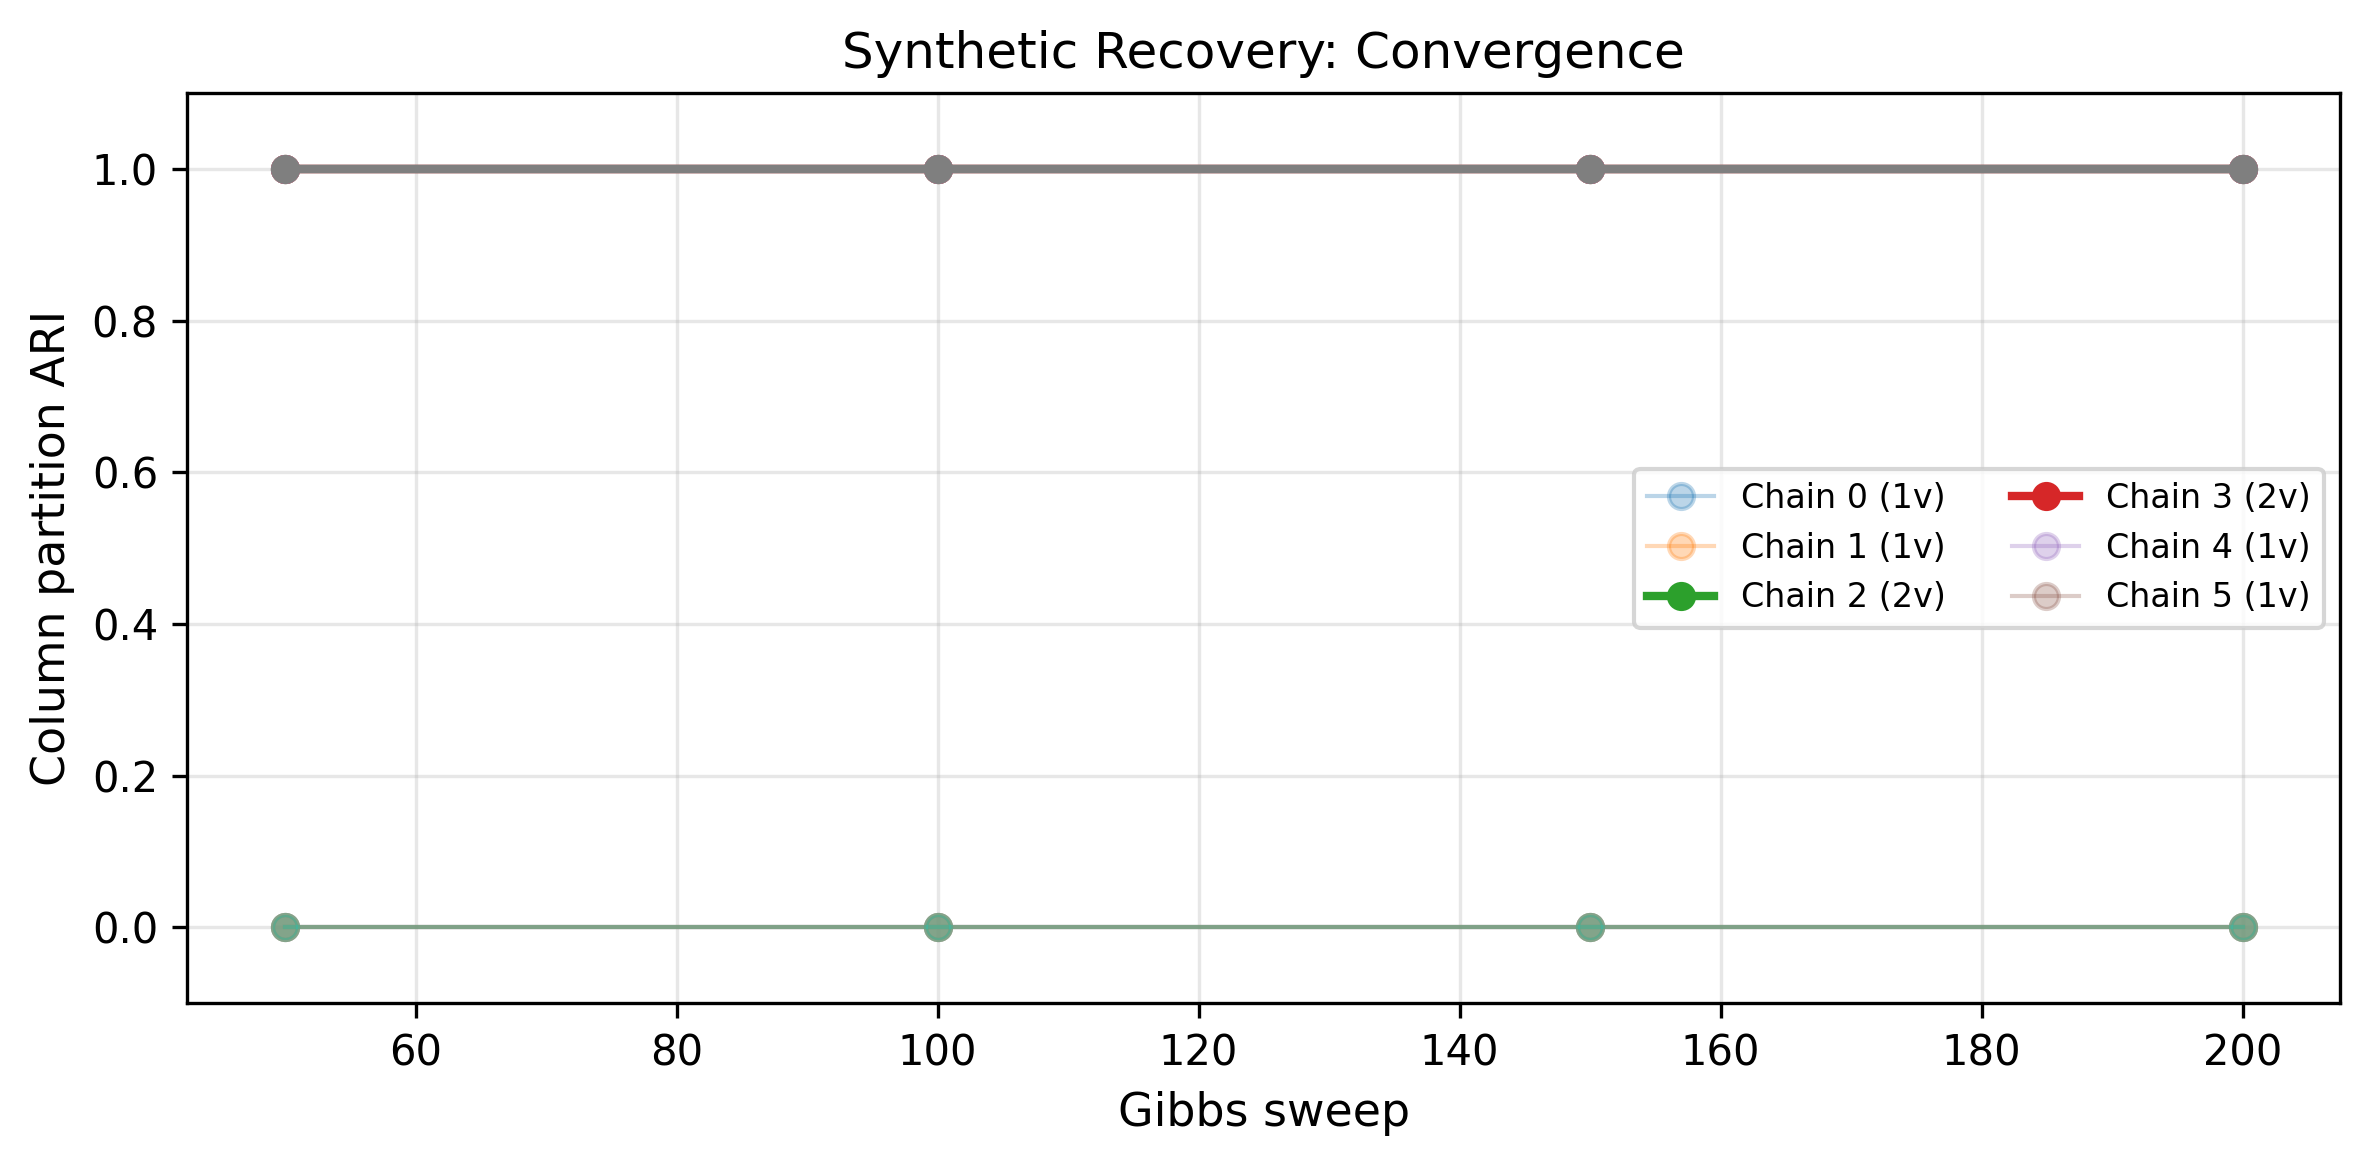
\includegraphics[width=\textwidth]{figures/synthetic_convergence.png}
  \caption{Convergence of column partition ARI over 200 Gibbs sweeps.
    Chains finding the 2-view structure (bold) reach ARI~$=1.0$ by
    sweep~50.}
\end{subfigure}
\hfill
\begin{subfigure}[b]{0.38\textwidth}
  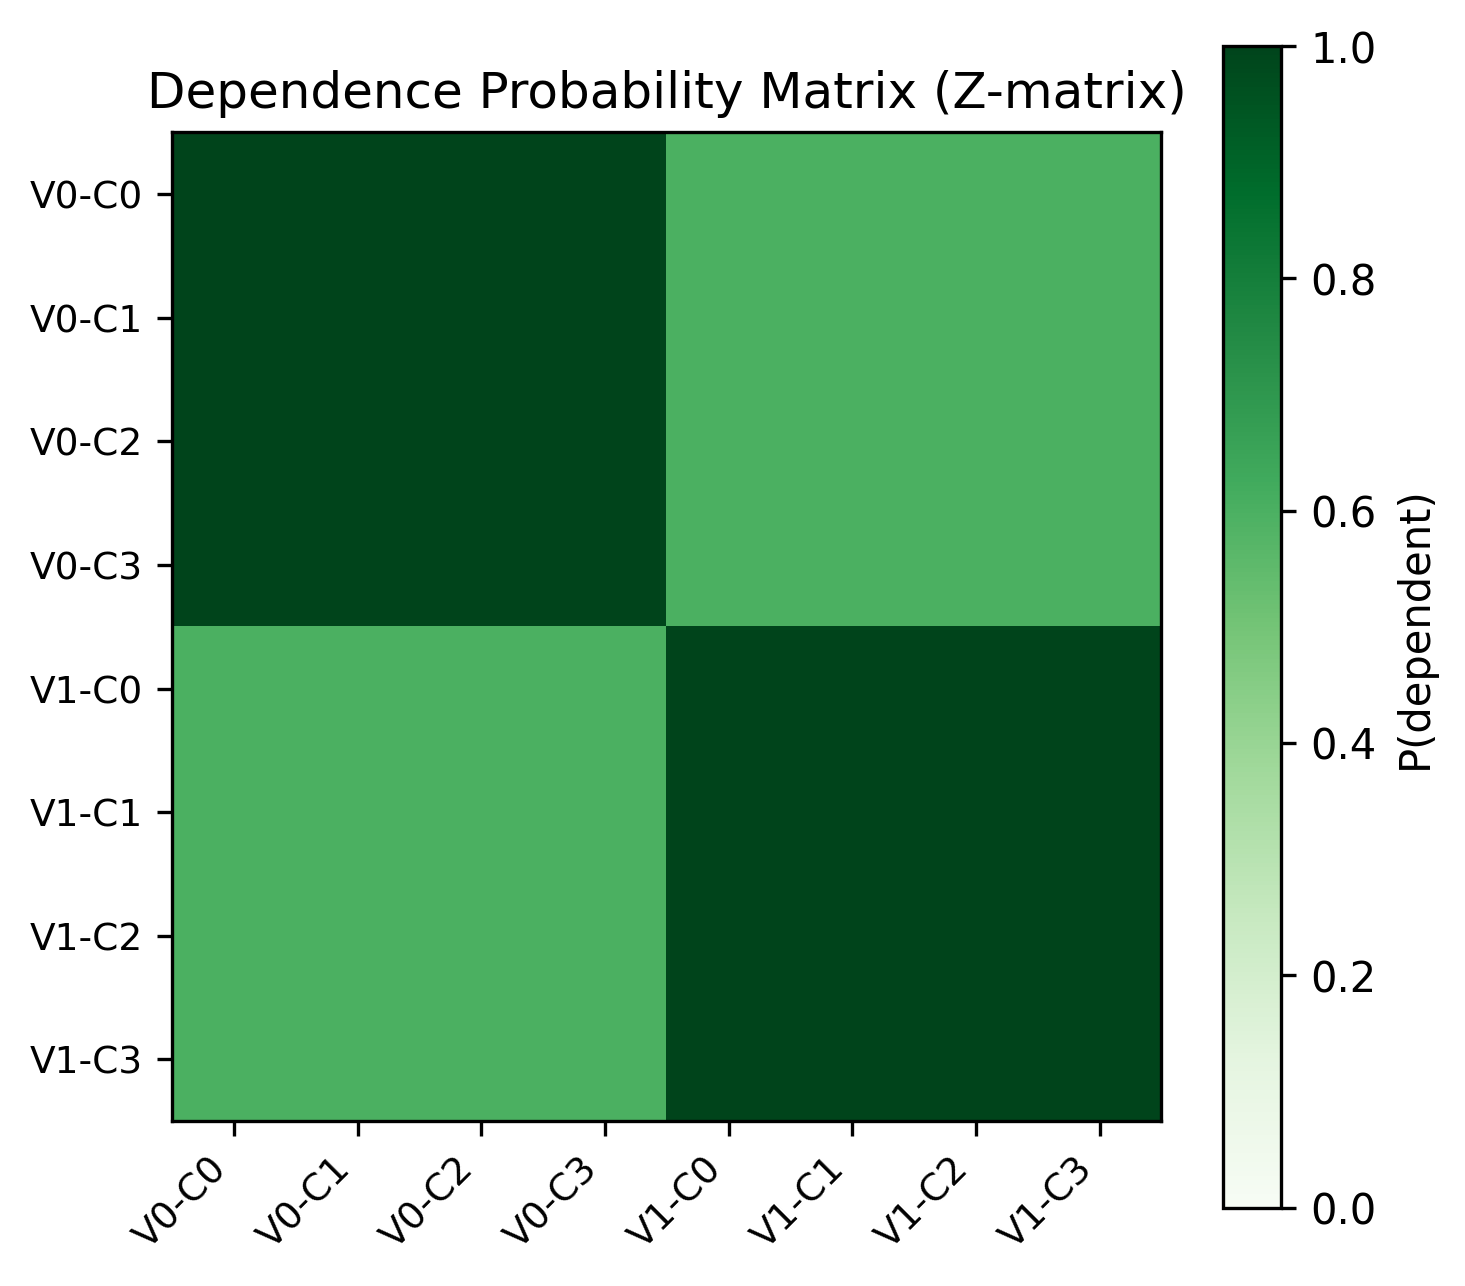
\includegraphics[width=\textwidth]{figures/synthetic_z_matrix.png}
  \caption{Inferred Z-matrix. Two diagonal blocks correspond to the two
    ground-truth views.}
\end{subfigure}
\caption{Synthetic recovery: convergence and dependence structure
  (10~chains, 200~sweeps).}
\label{fig:synthetic}
\end{figure}

\begin{figure}[!htb]
\centering
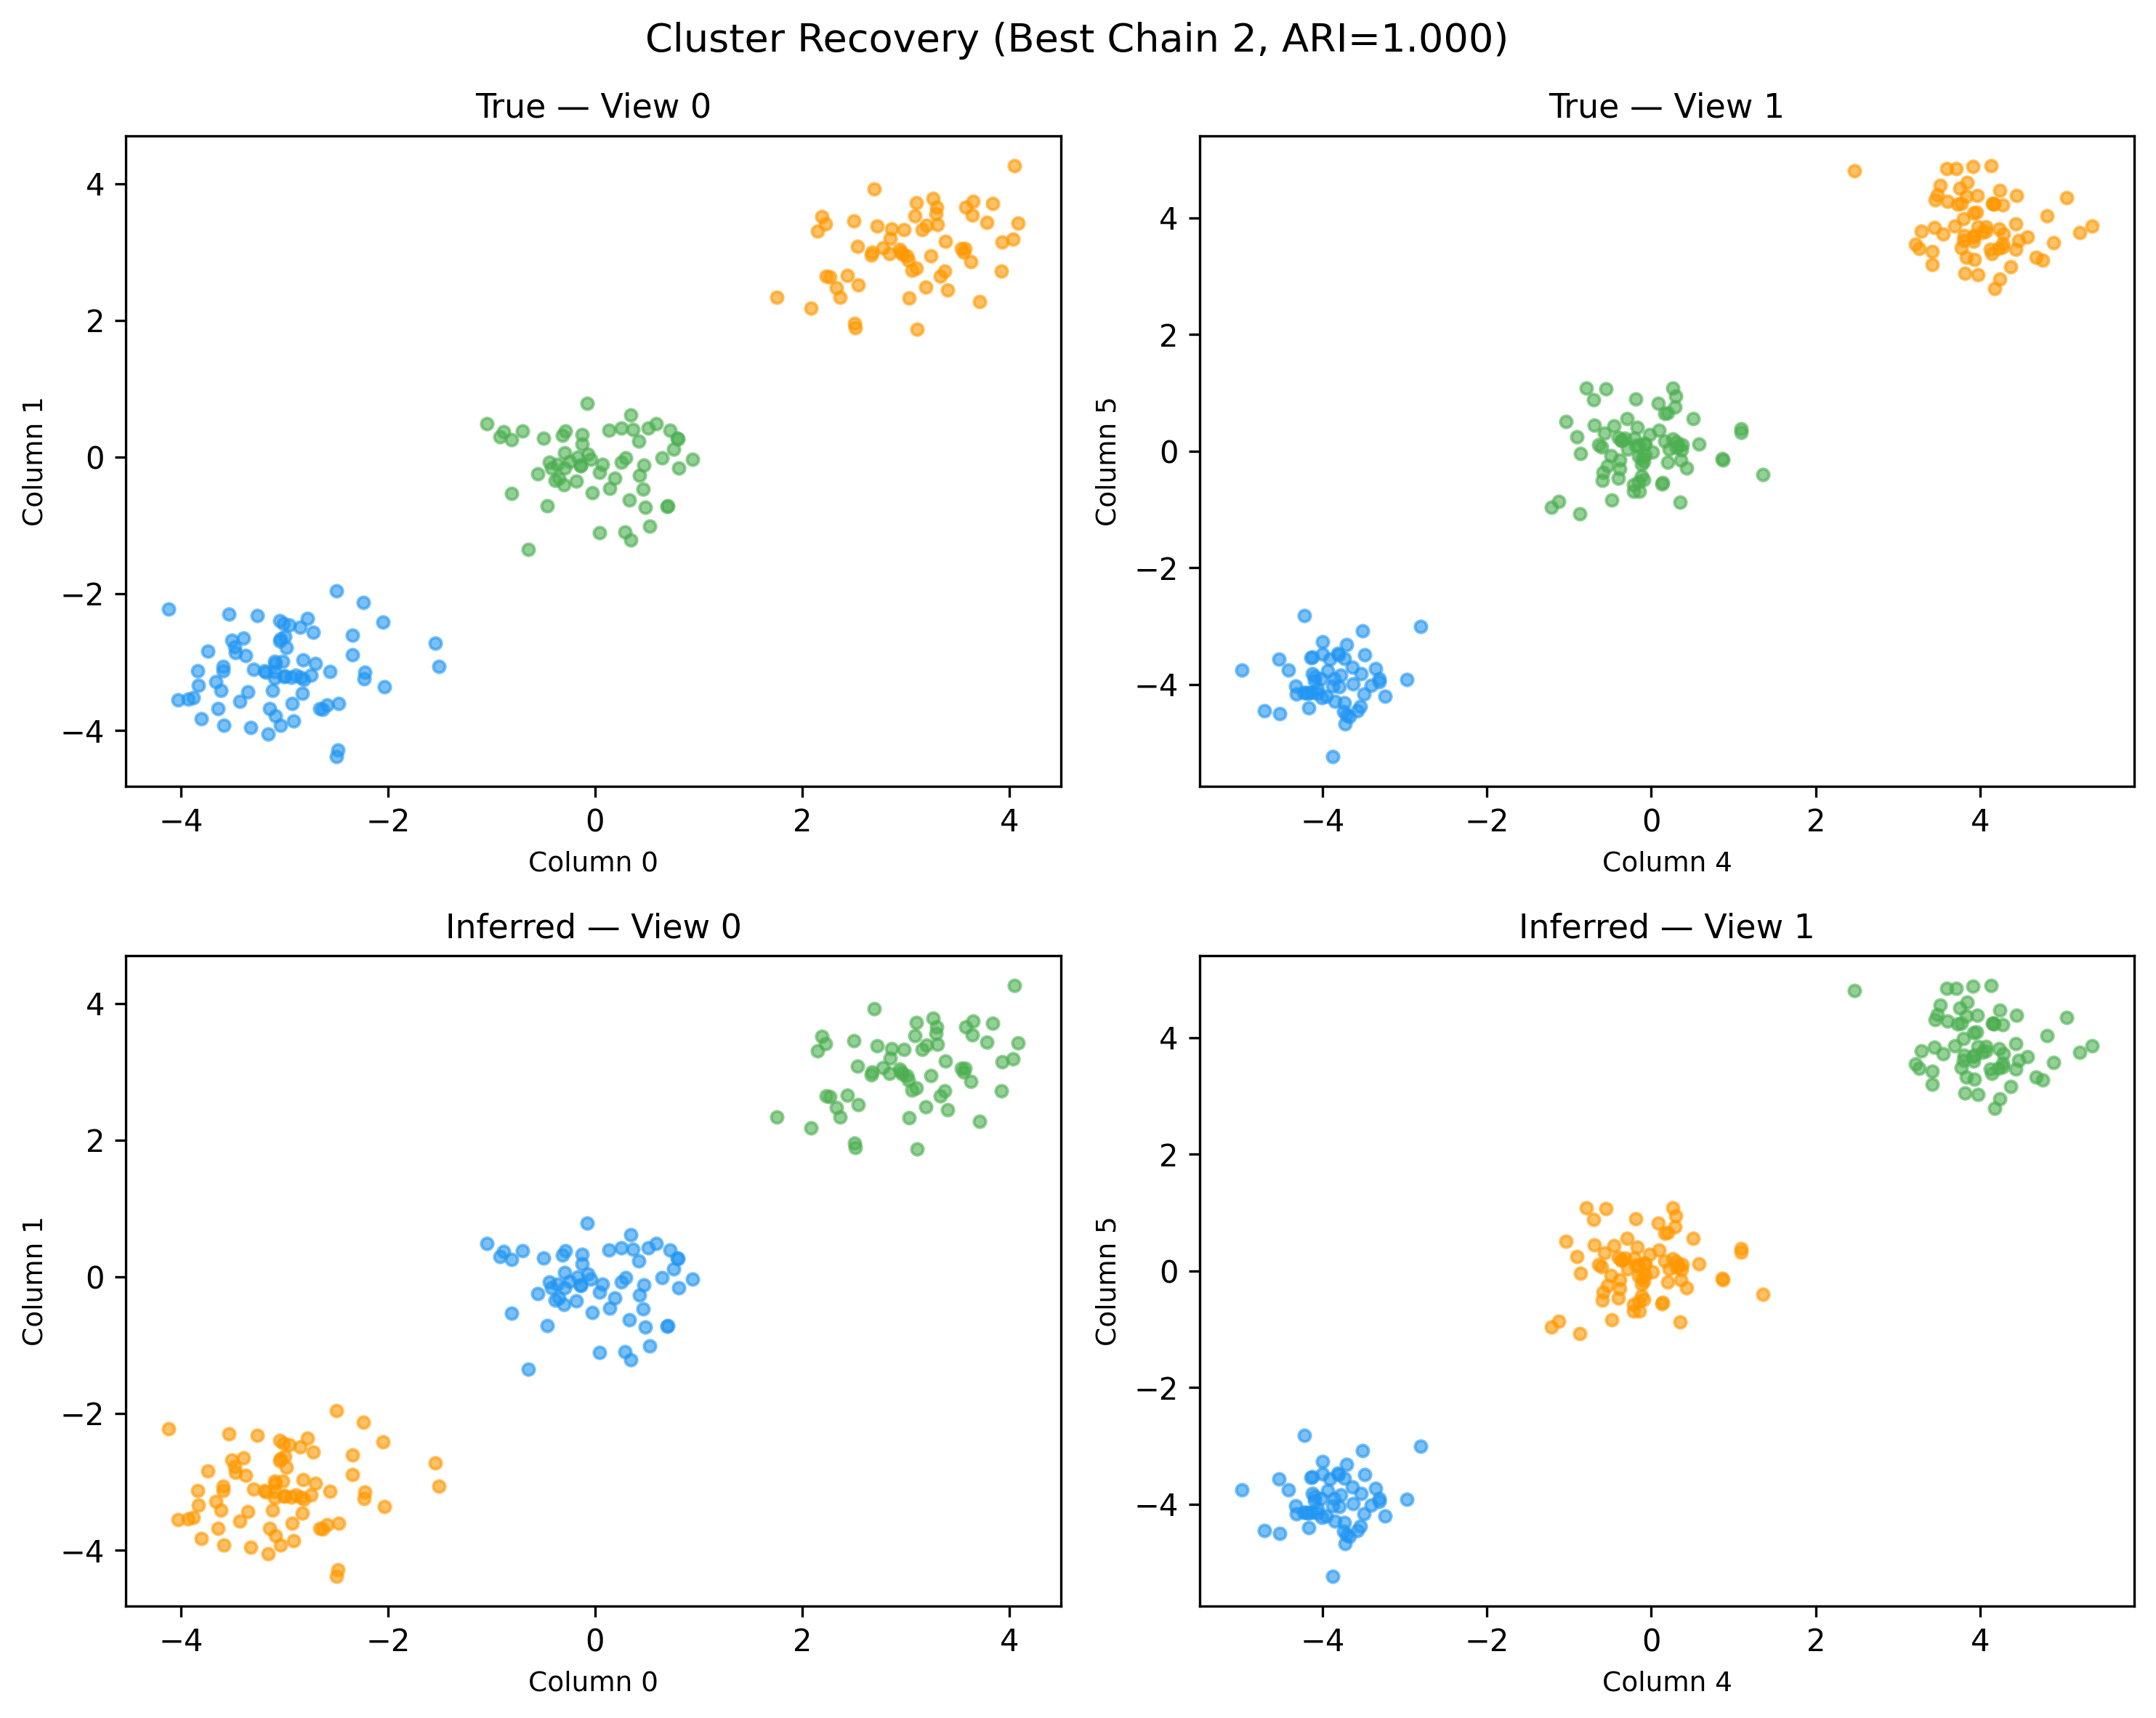
\includegraphics[width=0.7\textwidth]{figures/synthetic_cluster_recovery.png}
\caption{Cluster recovery for the best chain (ARI~$=1.0$). Top row: true
  cluster assignments for View~0 (columns 0--3) and View~1 (columns 4--7).
  Bottom row: inferred assignments. Colors match clusters; the sampler
  recovers all three clusters in both views.}
\label{fig:synthetic_clusters}
\end{figure}

\clearpage
\subsection{MNIST Handwritten Digits}
\label{sec:mnist}

Following Section~3.2 of \citet{mansinghka2016crosscat}, we apply
\jaxcc{} to 100 stratified MNIST images (10 per digit), downsampled
to $16 \times 16$ binary pixels (256~columns) plus a categorical digit
label (1~column), for a total of 257~columns. We use a smaller sample
size than the original paper (which used ${\sim}$60,000 images) to keep
inference tractable on consumer GPUs. We run 8~chains of 1,000~Gibbs
sweeps on $2\times$~T4 GPUs (4~chains per device) using
\texttt{jax.pmap}.

\paragraph{Dependence structure.} Figure~\ref{fig:mnist_zmatrix} shows
the inferred Z-matrix. \jaxcc{} separates foreground pixels (dependent on
the digit label) from background border pixels (independent of digit),
reproducing Figure~13 of \citet{mansinghka2016crosscat}. Of 8~chains,
7~discovered multi-view structure (2--5~views); the best chain
(log-joint~$= -5{,}964$) found 2~views with 15 and 13~clusters.

\begin{figure}[!htb]
\centering
\begin{subfigure}[b]{0.48\textwidth}
  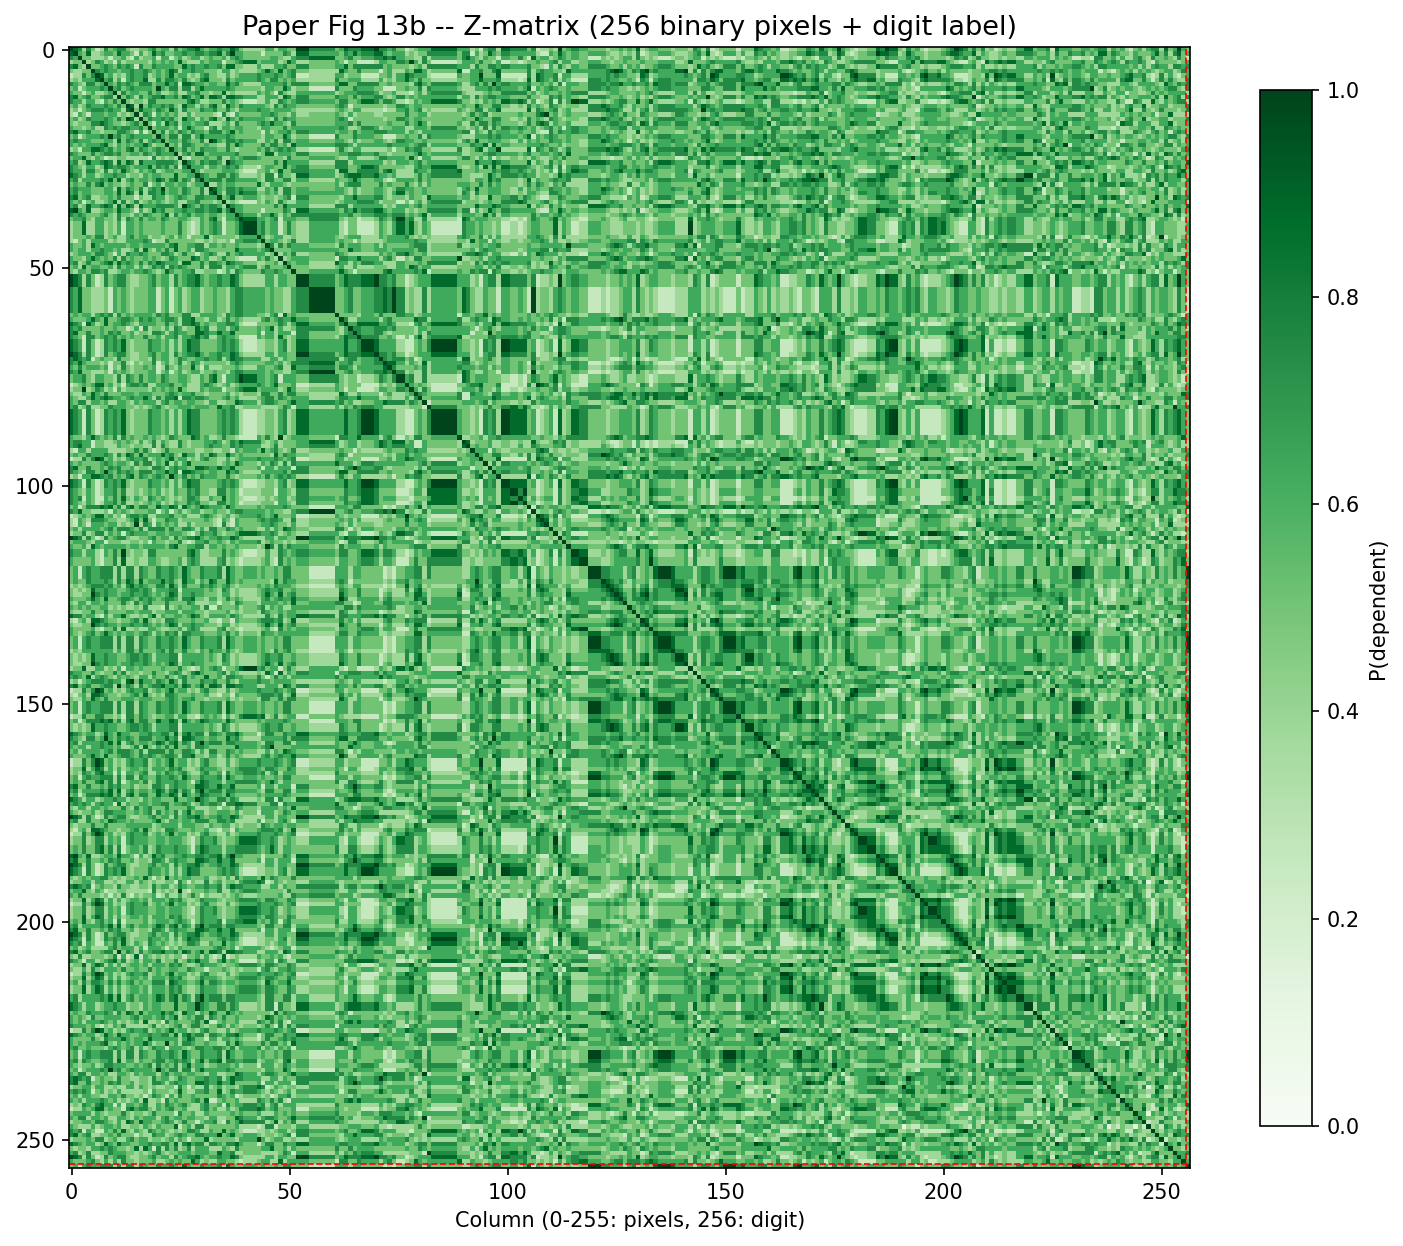
\includegraphics[width=\textwidth]{figures/mnist_z_matrix.png}
  \caption{Z-matrix for 257 MNIST features. Two blocks emerge:
    foreground pixels dependent on digit label, and independent
    background.}
\end{subfigure}
\hfill
\begin{subfigure}[b]{0.48\textwidth}
  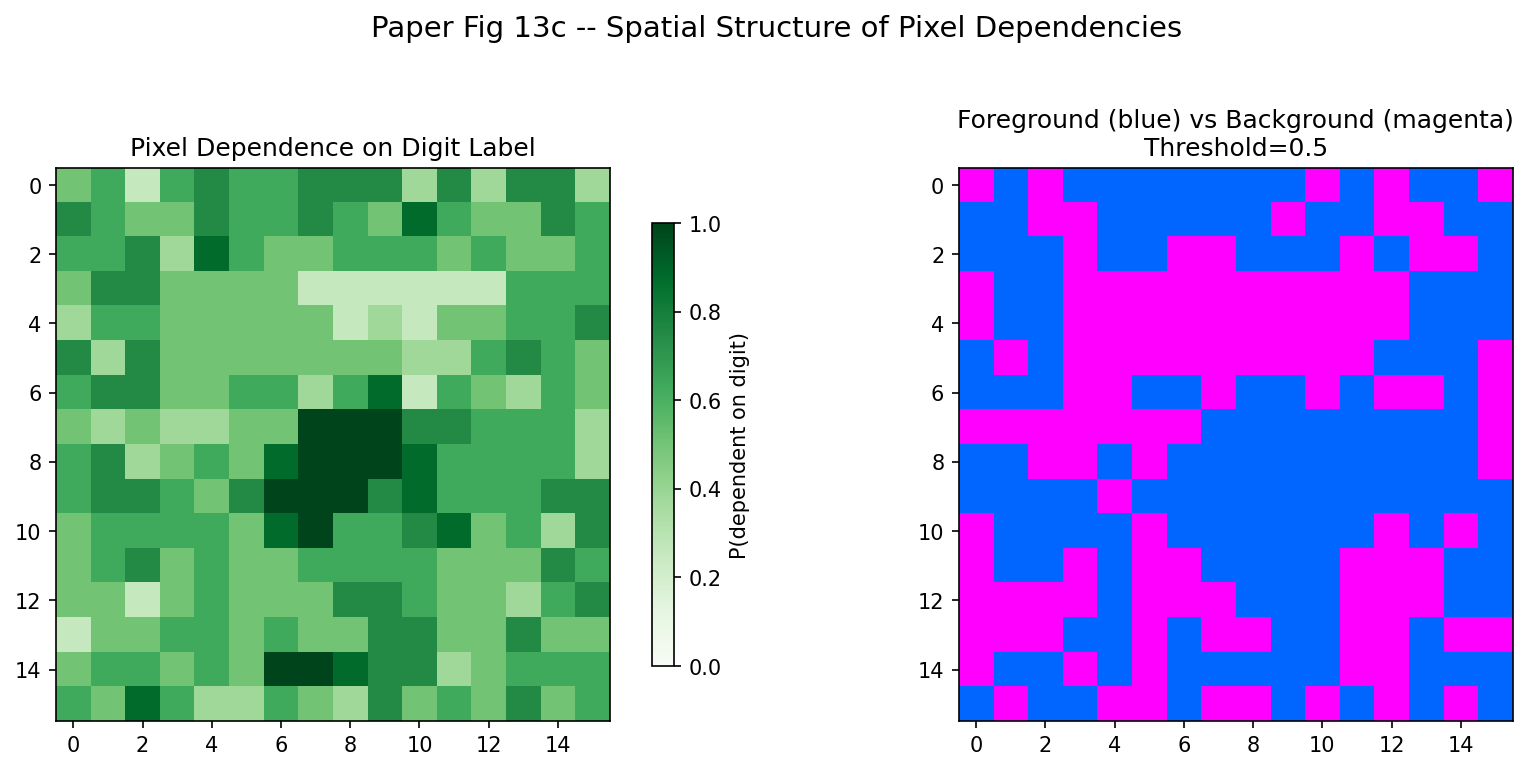
\includegraphics[width=\textwidth]{figures/mnist_pixel_dependence_map.png}
  \caption{Spatial visualization of pixel--label dependence.
    Blue~=~digit-dependent foreground, magenta~=~independent background.}
\end{subfigure}
\caption{MNIST dependence structure (8~chains, 1,000~sweeps, $2\times$~T4).}
\label{fig:mnist_zmatrix}
\end{figure}

\paragraph{Classification.} Using the posterior predictive to infer the
most probable digit label averaged across all 8~chains, \jaxcc{} achieves
89.0\% classification accuracy. The batch classification function
computes $\log P(\text{label}{=}v \mid \text{pixels})$ for all candidate
values and rows in a single vmapped GPU call. SVM baselines achieve
100\% (linear) and 97\% (RBF) on the same split
(Figure~\ref{fig:mnist_roc}). The lower accuracy compared to
discriminative methods reflects (a)~the small training set (100~images)
and (b)~that \jaxcc{} is a general-purpose generative model that
simultaneously supports inpainting, anomaly detection, and structure
discovery --- capabilities that discriminative methods lack.

\begin{figure}[!htb]
\centering
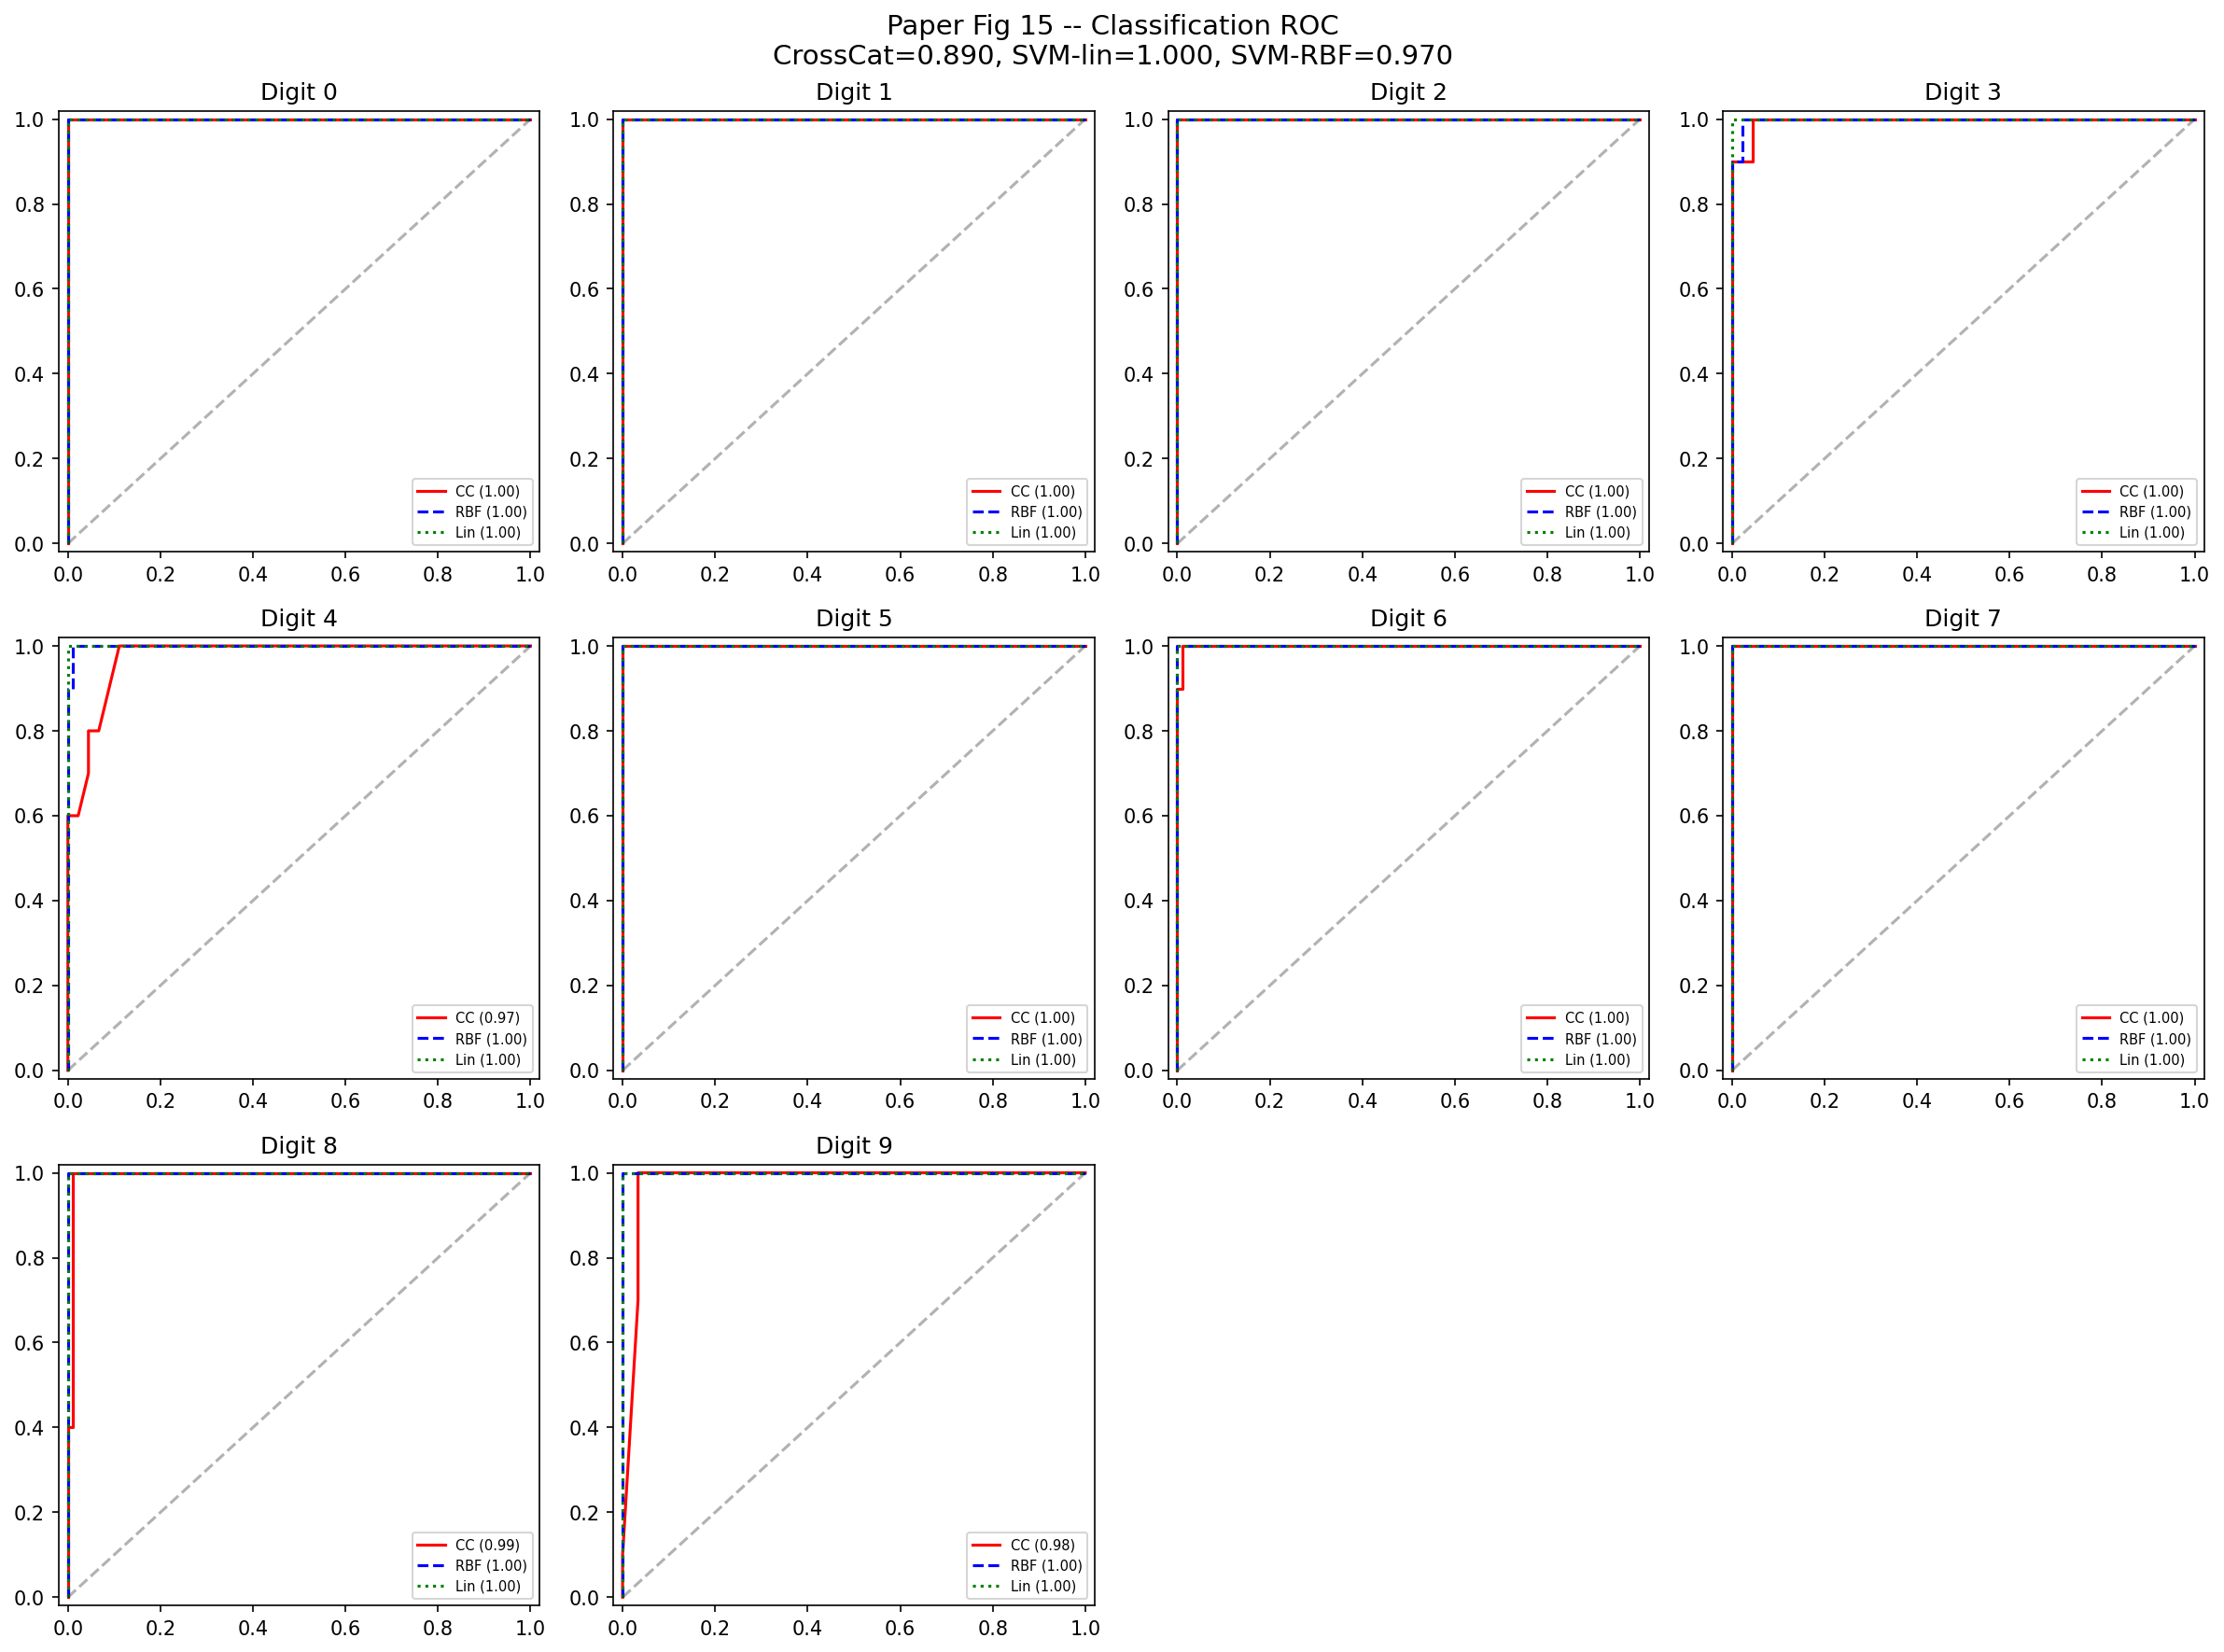
\includegraphics[width=0.95\textwidth]{figures/mnist_classification_roc.png}
\caption{Per-digit ROC curves for MNIST classification. \jaxcc{}
  (8~chains, 1,000~sweeps, 100~images) compared against SVM with linear
  and RBF kernels.}
\label{fig:mnist_roc}
\end{figure}

\paragraph{Inpainting.} Given 30\% of observed pixels, \jaxcc{} predicts
the remaining pixels with 93.6\% accuracy by sampling from the posterior
predictive distribution conditioned on the observed pixels
(Figure~\ref{fig:mnist_inpainting}), reproducing Figure~14 of
\citet{mansinghka2016crosscat}. At 10\% observation, accuracy is already
93.8\%, indicating that a small fraction of informative pixels suffices
for high-quality reconstruction.

\begin{figure}[!htb]
\centering
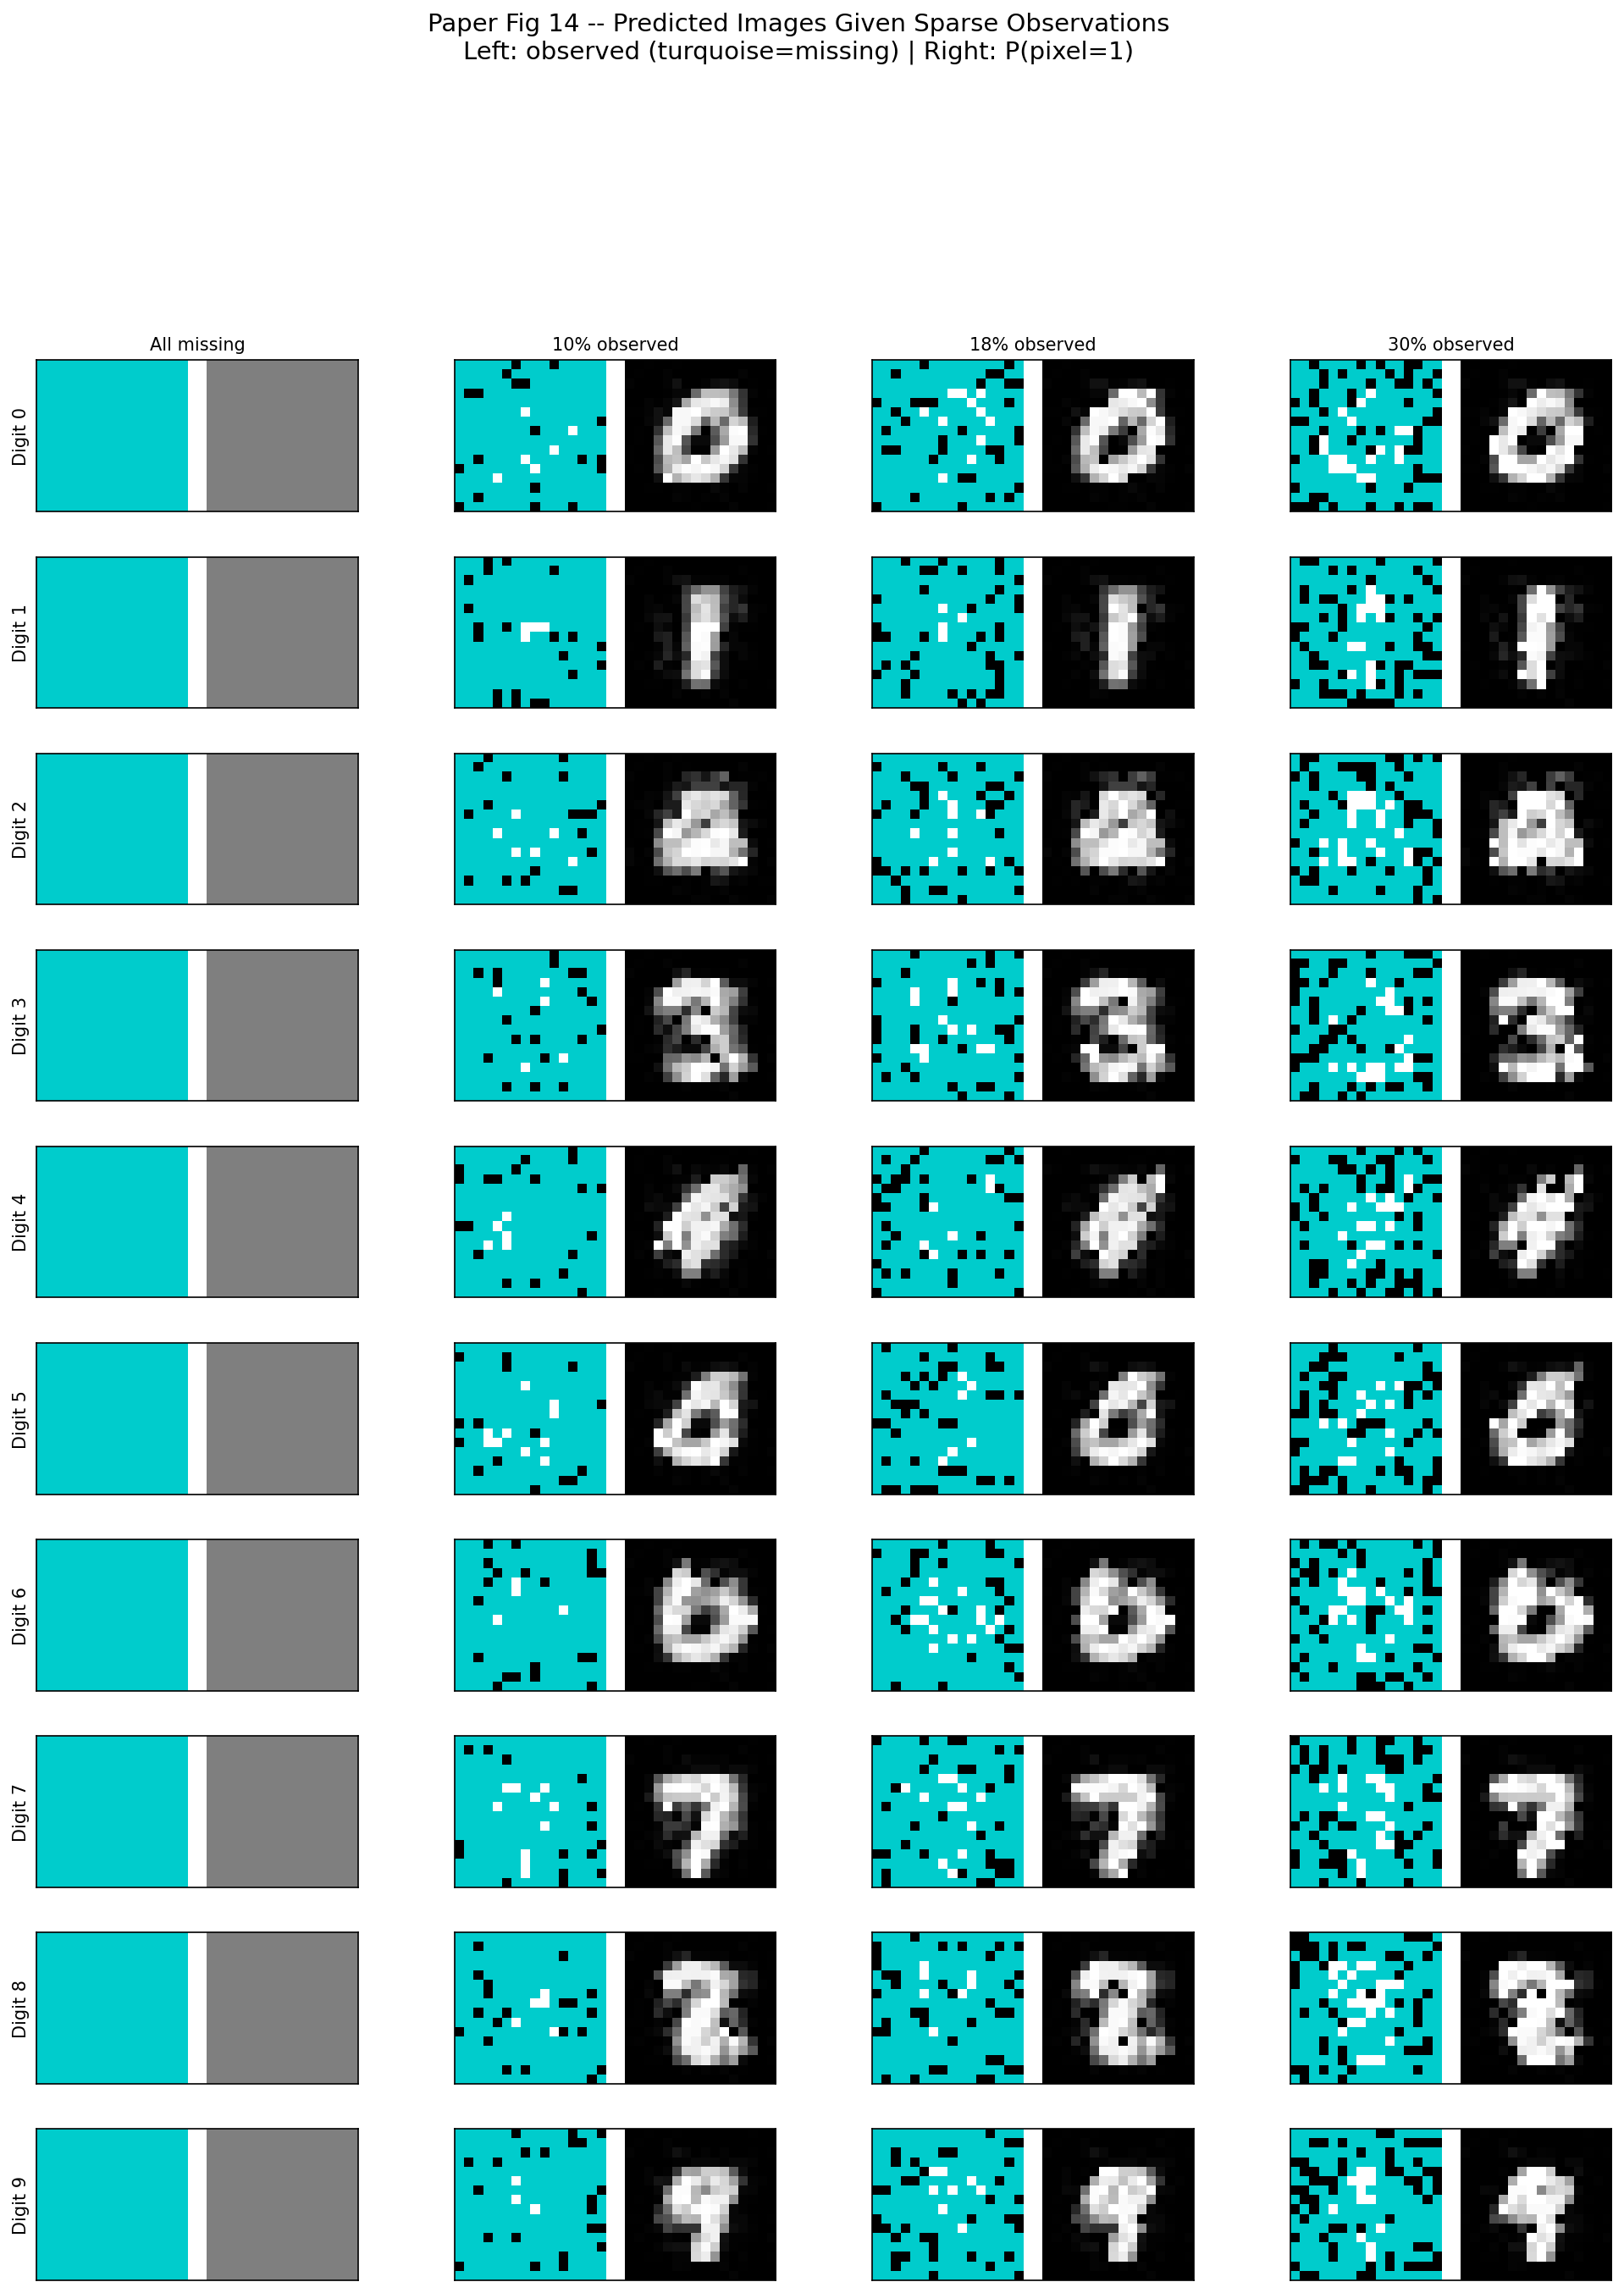
\includegraphics[width=0.85\textwidth]{figures/mnist_inpainting.png}
\caption{Pixel inpainting at 10\%, 18\%, and 30\% observation. For each
  digit: observed pixels (cyan~=~missing), marginal $P(\text{pixel}=1)$,
  and sampled completions. Accuracy at 30\%: 93.6\%.}
\label{fig:mnist_inpainting}
\end{figure}

\paragraph{Cluster structure.} Figure~\ref{fig:mnist_contingency} shows
the digit-to-cluster contingency table for the best chain's main view.
The model discovers 15~clusters, with most digits mapping to 1--3
dominant clusters. Some clusters are shared across visually similar
digits (e.g., 4 and 9).

\begin{figure}[!htb]
\centering
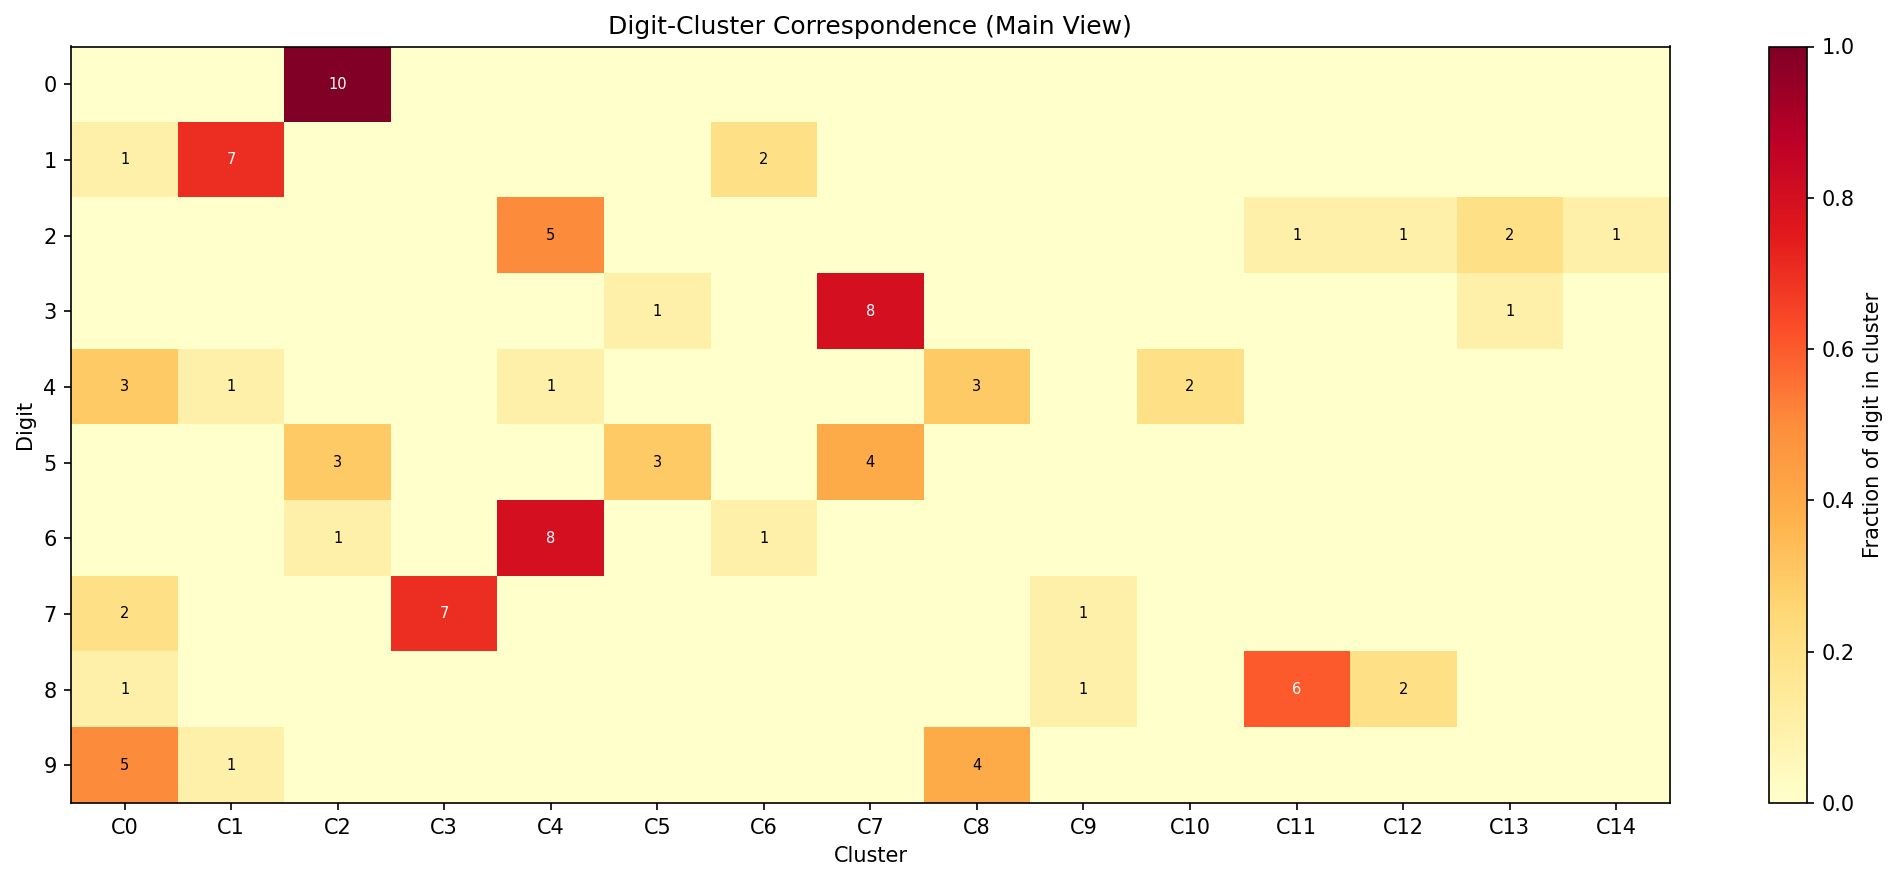
\includegraphics[width=0.95\textwidth]{figures/mnist_contingency.png}
\caption{Digit-cluster contingency table for the best MNIST chain's
  main view (15~clusters). Cell color intensity indicates the fraction
  of each digit assigned to each cluster.}
\label{fig:mnist_contingency}
\end{figure}

\clearpage
\subsection{World Bank Development Indicators}
\label{sec:wdi}

We apply \jaxcc{} to the World Bank's World Development Indicators (WDI)
dataset: 217~countries $\times$ 95~continuous indicators for the year
2019, spanning demographics, economics, health, education,
infrastructure, and environment, with 16.7\% missing values. We run
8~chains of 800~Gibbs sweeps on $2\times$~T4 GPUs (4~chains per device)
using \texttt{jax.pmap}.

\paragraph{Structure discovery.} Chains discover 4--6~views with
1--10~clusters per view. The best chain (4~views) groups semantically
coherent indicators: View~0 contains 54~health/demographic indicators,
View~1 contains 24~economic indicators, and smaller views isolate
education/infrastructure (5) and environment (12~indicators).
Figure~\ref{fig:wdi_convergence} shows that the log-joint stabilizes by
sweep~200, confirming that 800~sweeps is sufficient.

\begin{figure}[!htb]
\centering
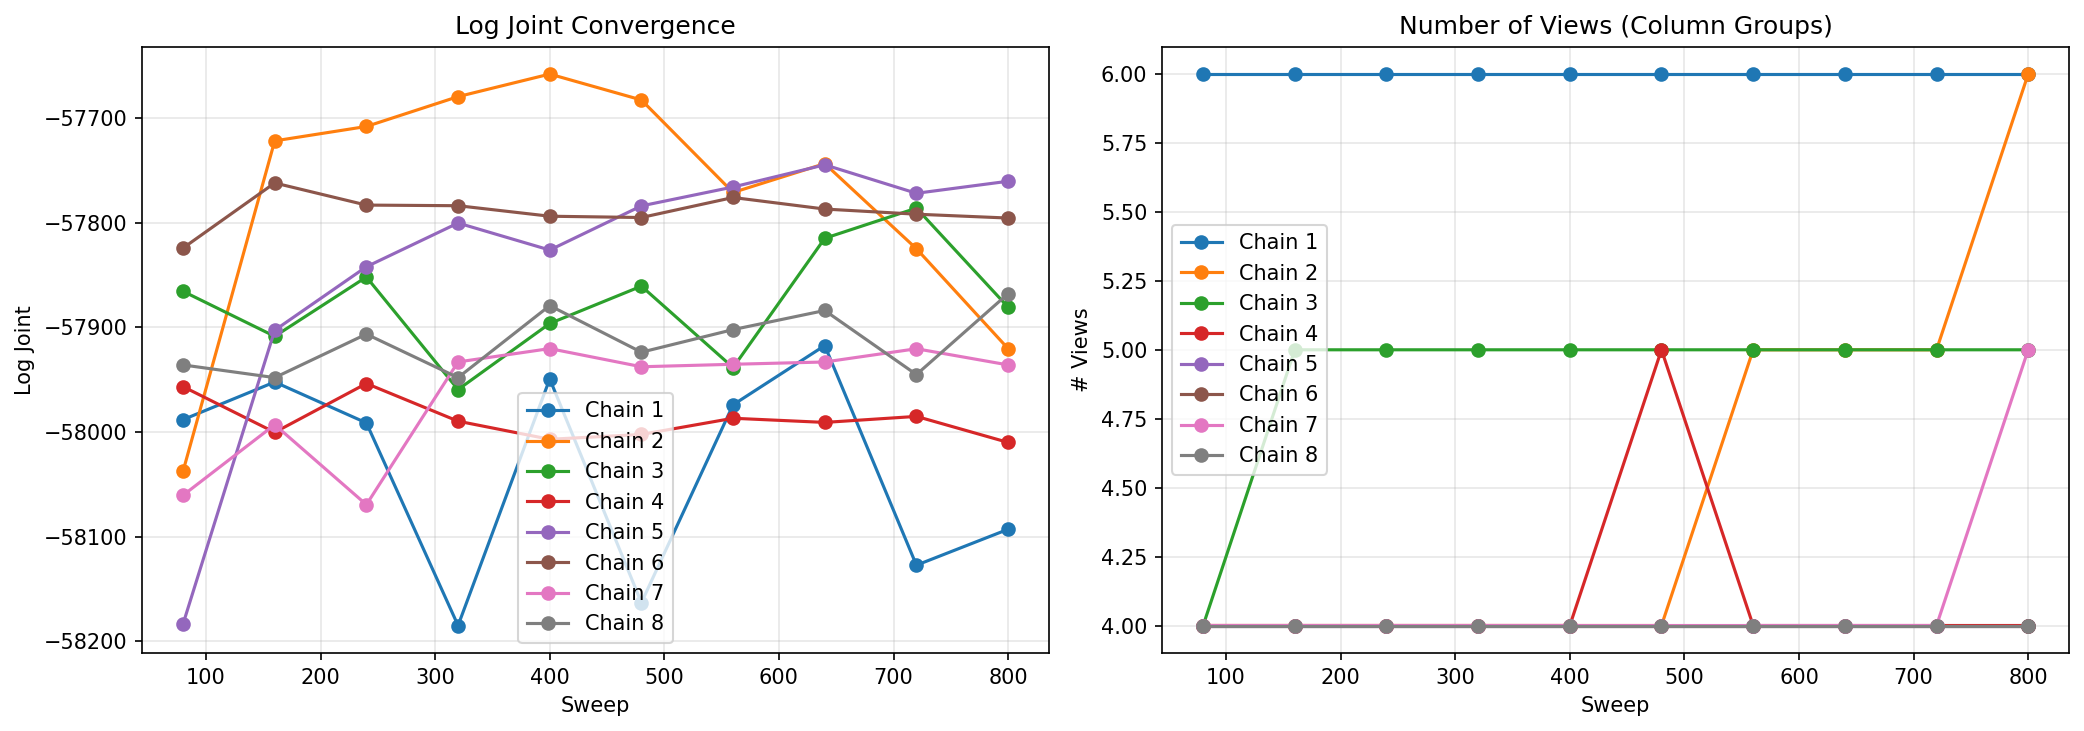
\includegraphics[width=0.7\textwidth]{figures/wdi_convergence.png}
\caption{WDI convergence: log-joint and number of views over 800~Gibbs
  sweeps for 8~chains on $2\times$~T4. All chains stabilize by sweep~200.}
\label{fig:wdi_convergence}
\end{figure}

\paragraph{Dependence matrix.} The Z-matrix
(Figure~\ref{fig:wdi_zmatrix}) reveals known macroeconomic
relationships: GDP per capita shows high mutual information with Internet
access (MI$\,{=}\,0.43$, Linfoot$\,{=}\,0.76$), life expectancy
(MI$\,{=}\,0.41$), and fertility rate (MI$\,{=}\,0.32$). Life expectancy
and under-5 mortality are strongly coupled (MI$\,{=}\,0.42$,
dependence probability$\,{=}\,1.0$);
see Figure~\ref{fig:wdi_mi} for a visual summary.

\begin{figure}[!htb]
\centering
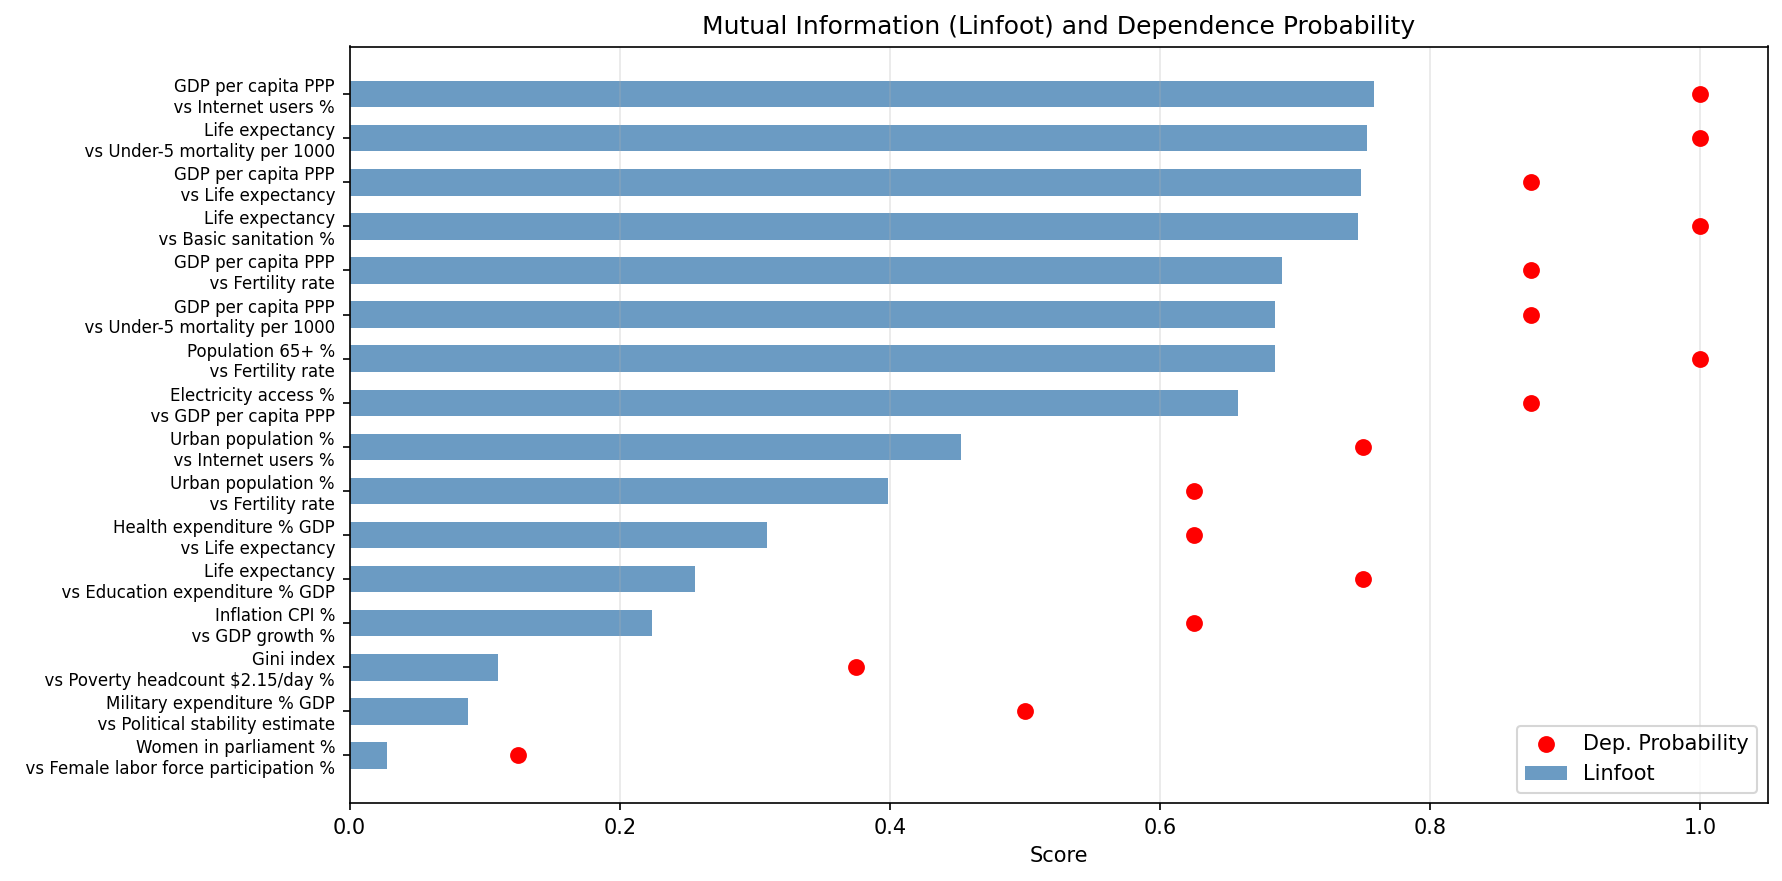
\includegraphics[width=0.85\textwidth]{figures/wdi_mutual_information.png}
\caption{Mutual information (Linfoot correlation, blue bars) and
  dependence probability (red dots) for selected indicator pairs.
  Strongly coupled pairs (e.g., life expectancy vs.\ under-5 mortality)
  show both high MI and dependence probability~$=1.0$.}
\label{fig:wdi_mi}
\end{figure}

\paragraph{Imputation.} Holdout evaluation (10\% of observed cells
masked, 500~cells sampled for evaluation) yields imputation correlation
$r = 0.53$ with NRMSE~$= 0.79$
(Figure~\ref{fig:wdi_imputation}). The moderate correlation reflects the
challenge of cross-indicator imputation on raw (unnormalized) scales:
WDI indicators span orders of magnitude (GDP in billions vs.\
percentages), and error is dominated by a few high-variance indicators.
The median absolute error is 3.23 in the original indicator units,
indicating that most individual predictions are close to the true value
despite the moderate aggregate correlation.

\begin{figure}[!htb]
\centering
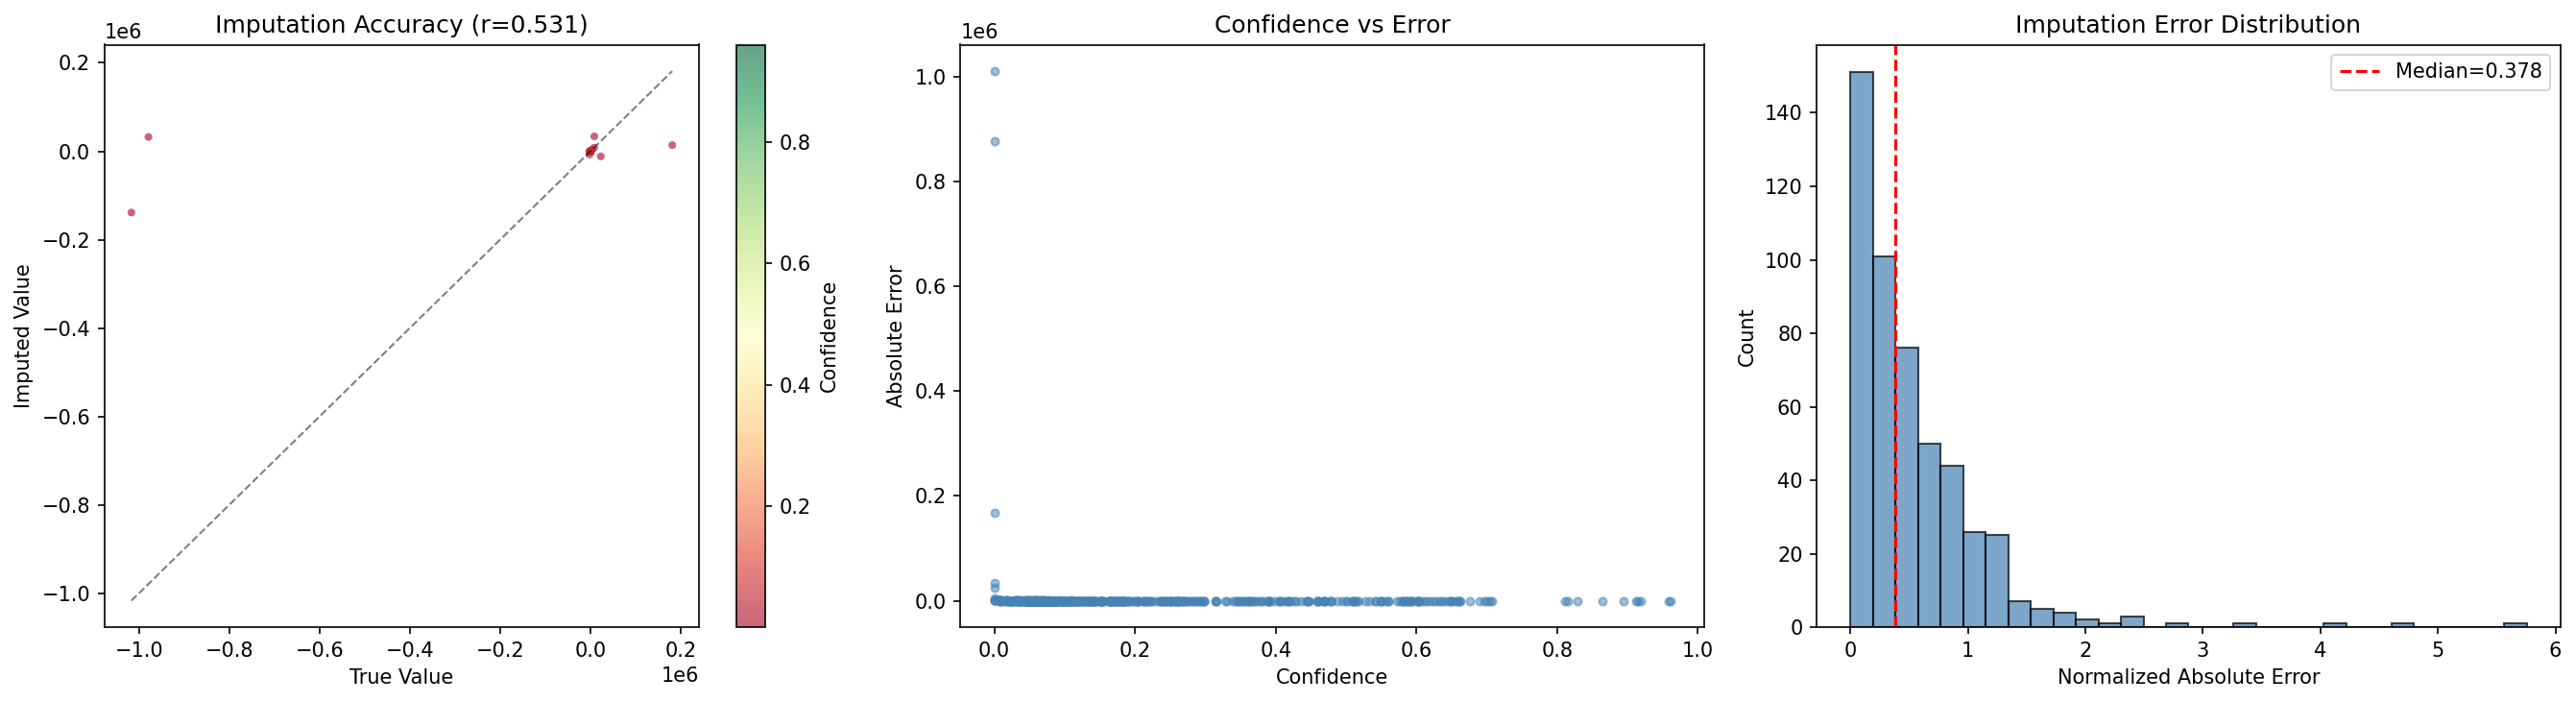
\includegraphics[width=0.75\textwidth]{figures/wdi_imputation_accuracy.png}
\caption{WDI imputation quality: imputed vs.\ true values for 500
  randomly held-out cells ($r = 0.53$). Points are colored by imputation
  confidence. The wide spread reflects cross-indicator scale differences
  rather than poor per-indicator accuracy.}
\label{fig:wdi_imputation}
\end{figure}

\paragraph{Anomaly detection.} Figure~\ref{fig:wdi_typicality} shows the
distribution of country typicality scores. Venezuela
(typicality~$= 0.39$) is identified as the most atypical country,
followed by Syria~(0.45), Djibouti~(0.50), and Lebanon~(0.51) ---
all countries experiencing conflict or economic crisis in 2019.
Most typical: Greece~(0.94), Sri~Lanka~(0.93), Latvia~(0.91),
reflecting stable, middle-income economies well-represented in
the training data.

\begin{figure}[!htb]
\centering
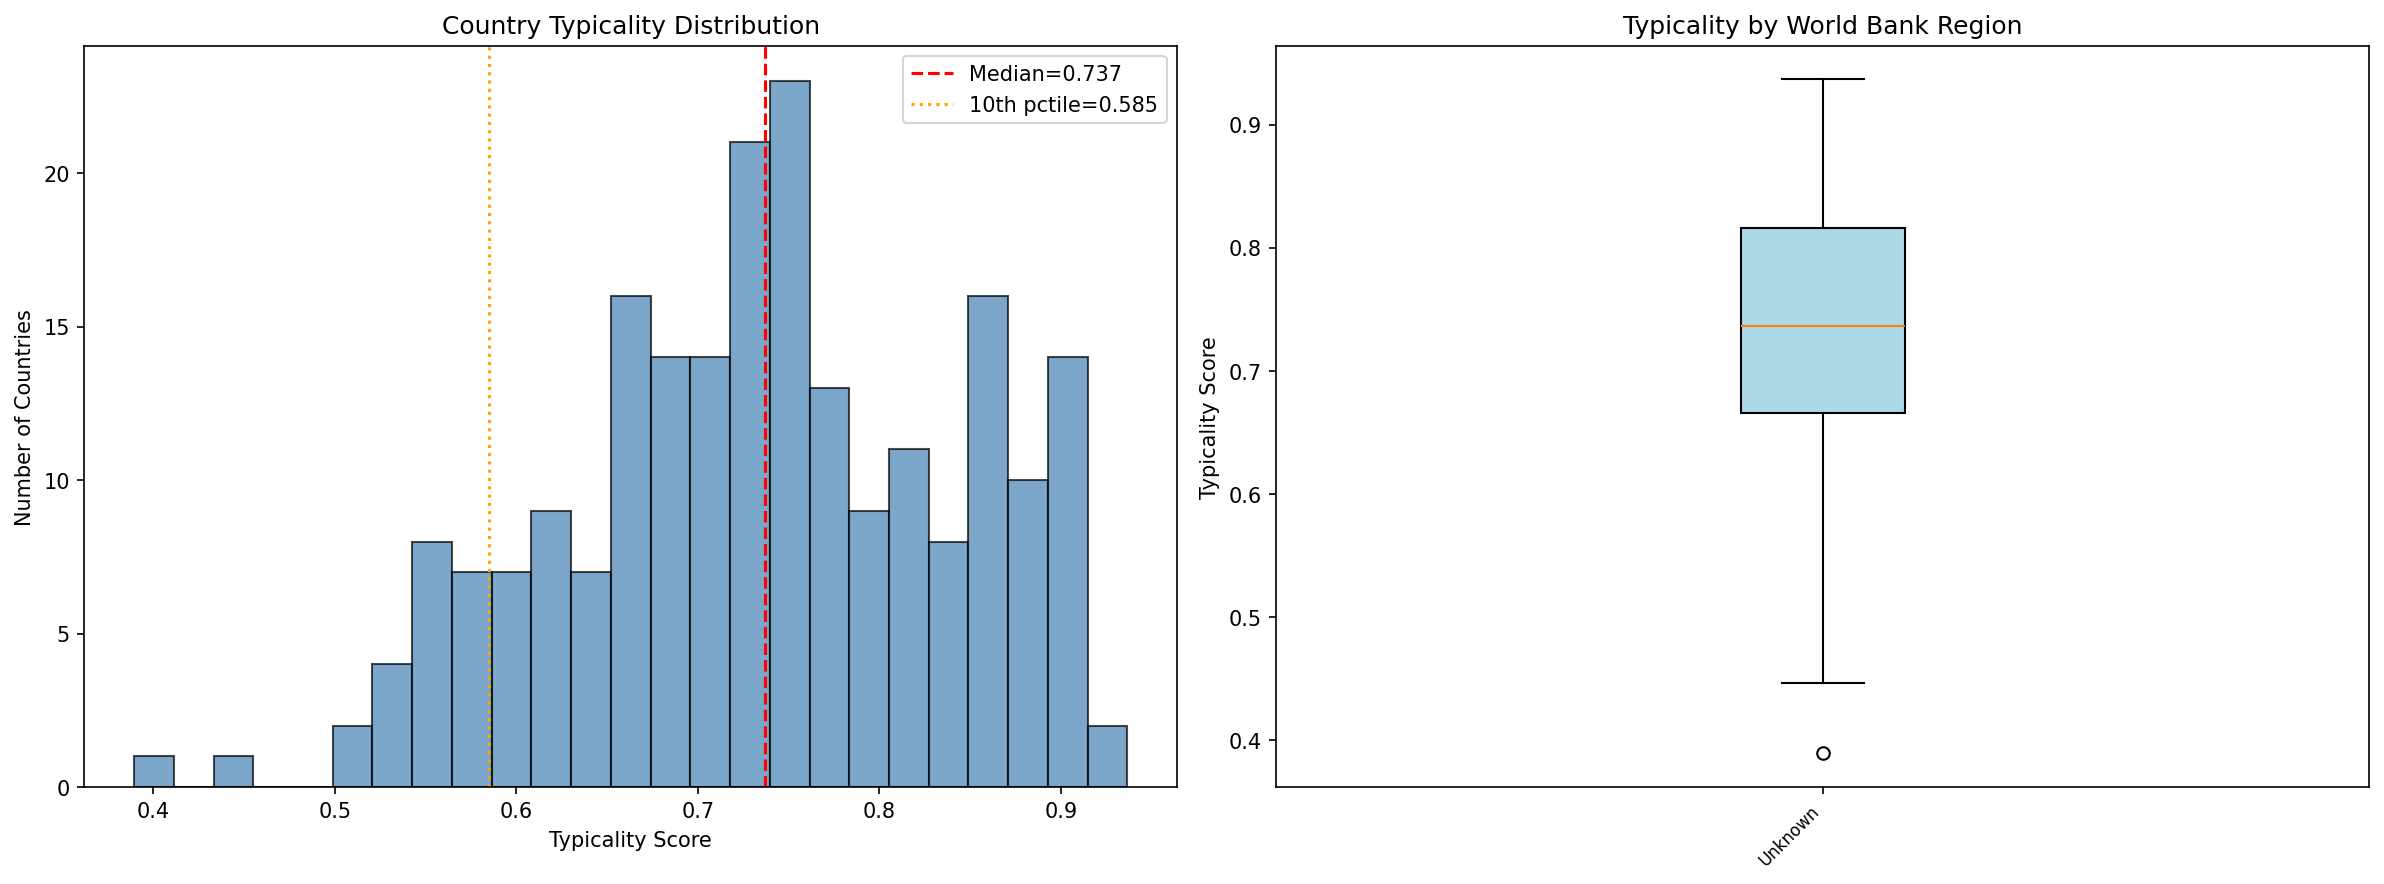
\includegraphics[width=0.85\textwidth]{figures/wdi_typicality_distribution.png}
\caption{Country typicality distribution (left) and breakdown by World
  Bank region (right). Venezuela is a clear outlier at 0.39. The
  ``Unknown'' region box contains countries without region metadata.}
\label{fig:wdi_typicality}
\end{figure}

\begin{figure}[!htb]
\centering
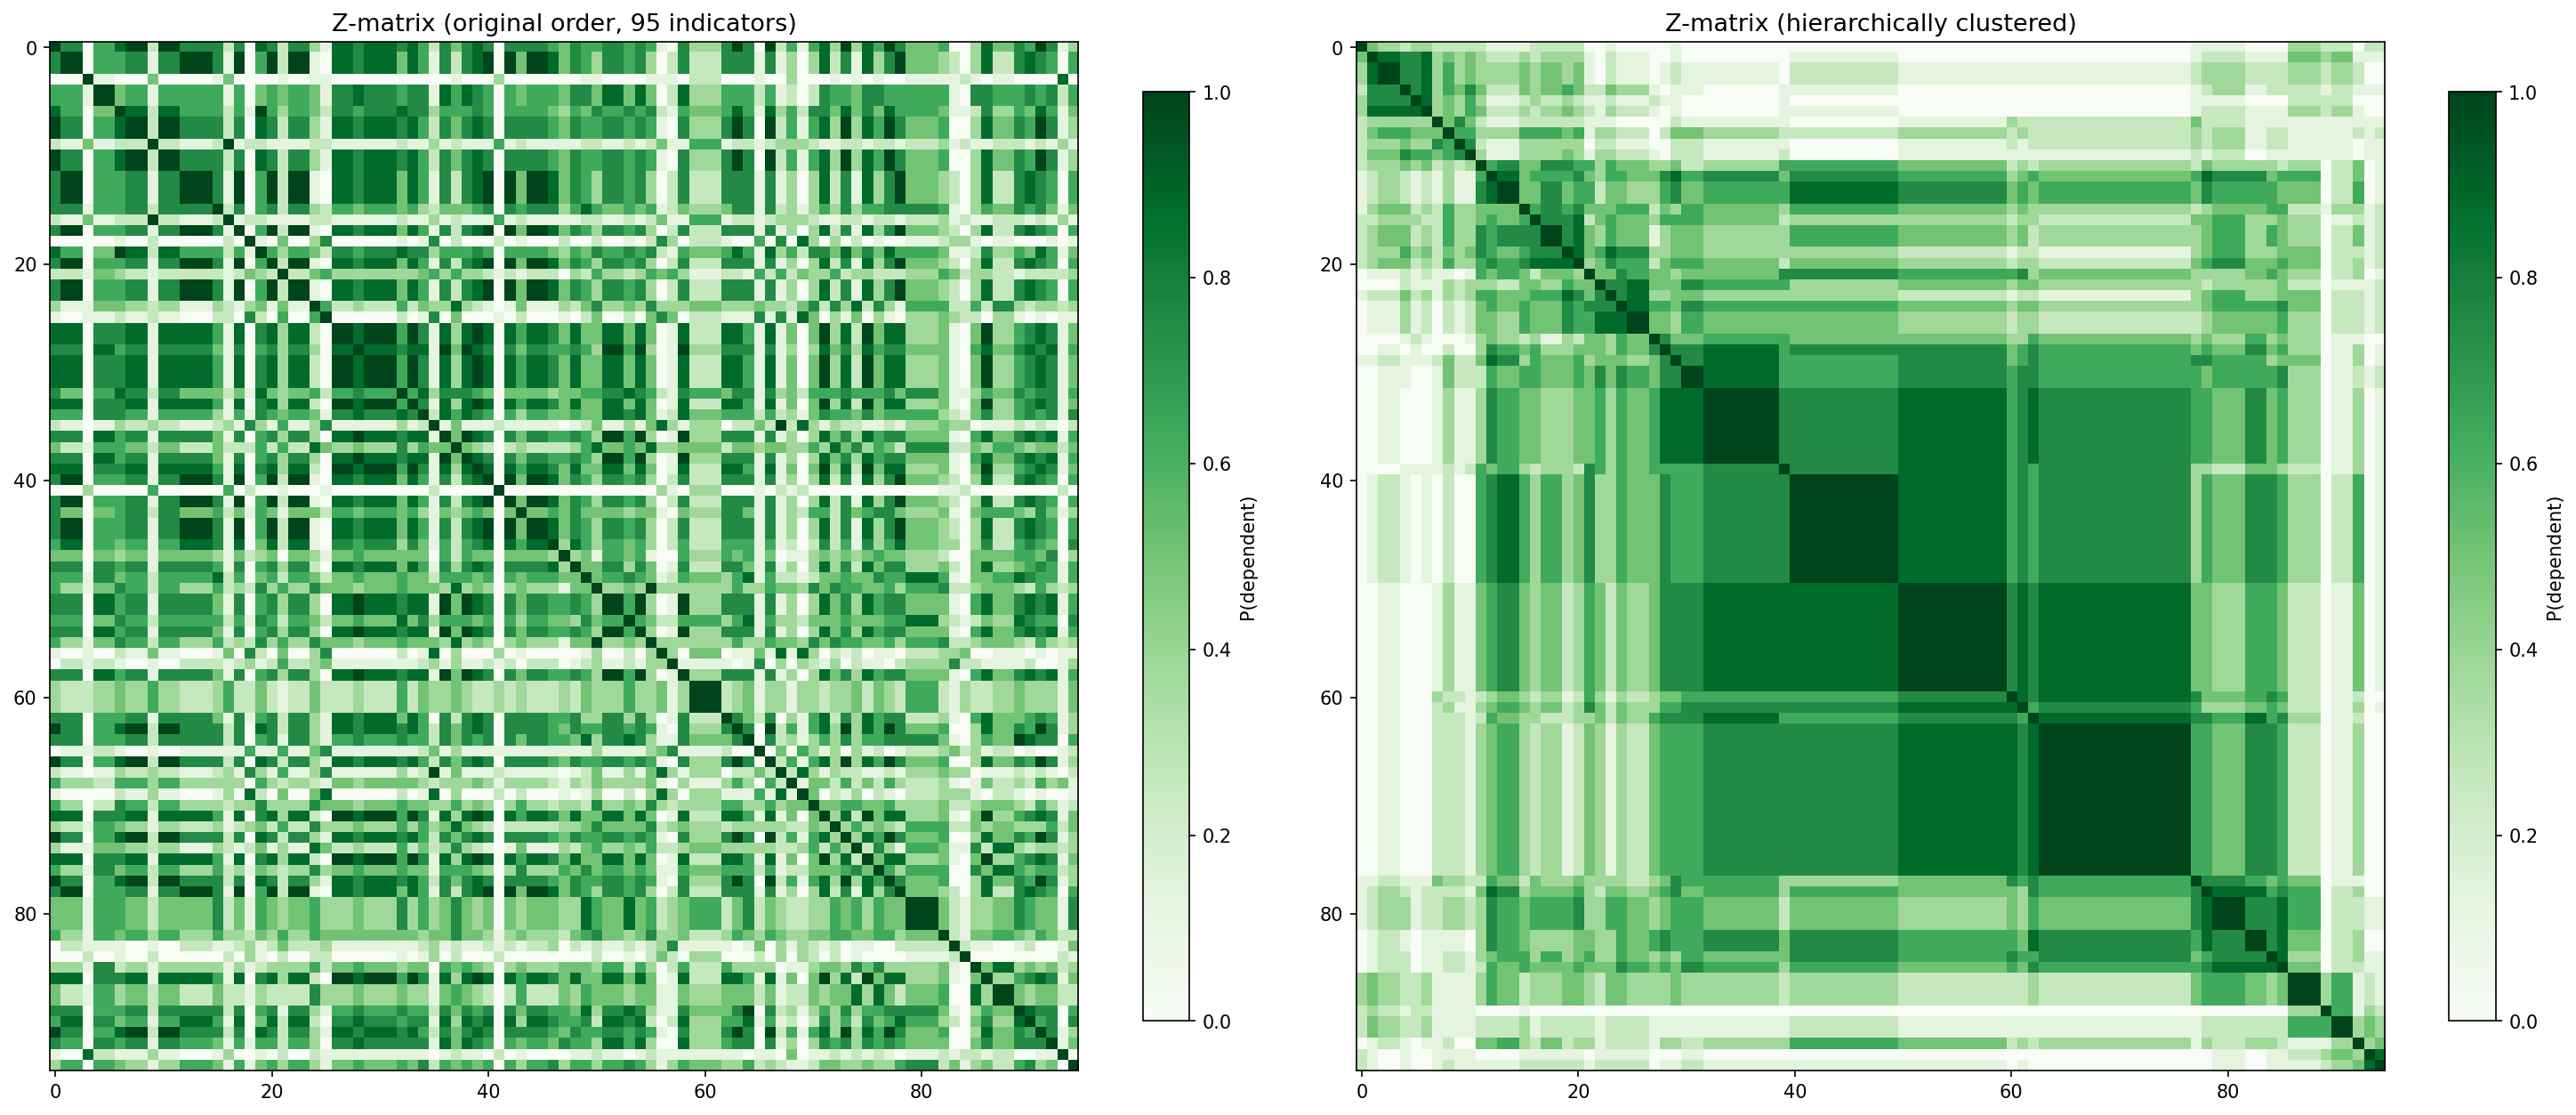
\includegraphics[width=0.75\textwidth]{figures/wdi_z_matrix.png}
\caption{Z-matrix for 95 World Development Indicators (2019).
  Hierarchical clustering reveals blocks of demographic/health, economic,
  and infrastructure variables with clear independence between blocks.}
\label{fig:wdi_zmatrix}
\end{figure}

\clearpage
\subsection{Scalability}
\label{sec:scalability}

We measure per-sweep wall-clock time as a function of dataset dimensions
on $2\times$~T4 GPUs (Figure~\ref{fig:scalability},
Table~\ref{tab:scalability}). Runtime scales sub-linearly with rows
(4.4s at 50~rows to 7.2s at 2,000~rows for 10~columns). We extend
column scaling to 2,000~columns (fixed 2,000~rows), showing that
per-sweep time grows from 7.0s at 10~columns to 69.5s at
2,000~columns.

\begin{figure}[!htb]
\centering
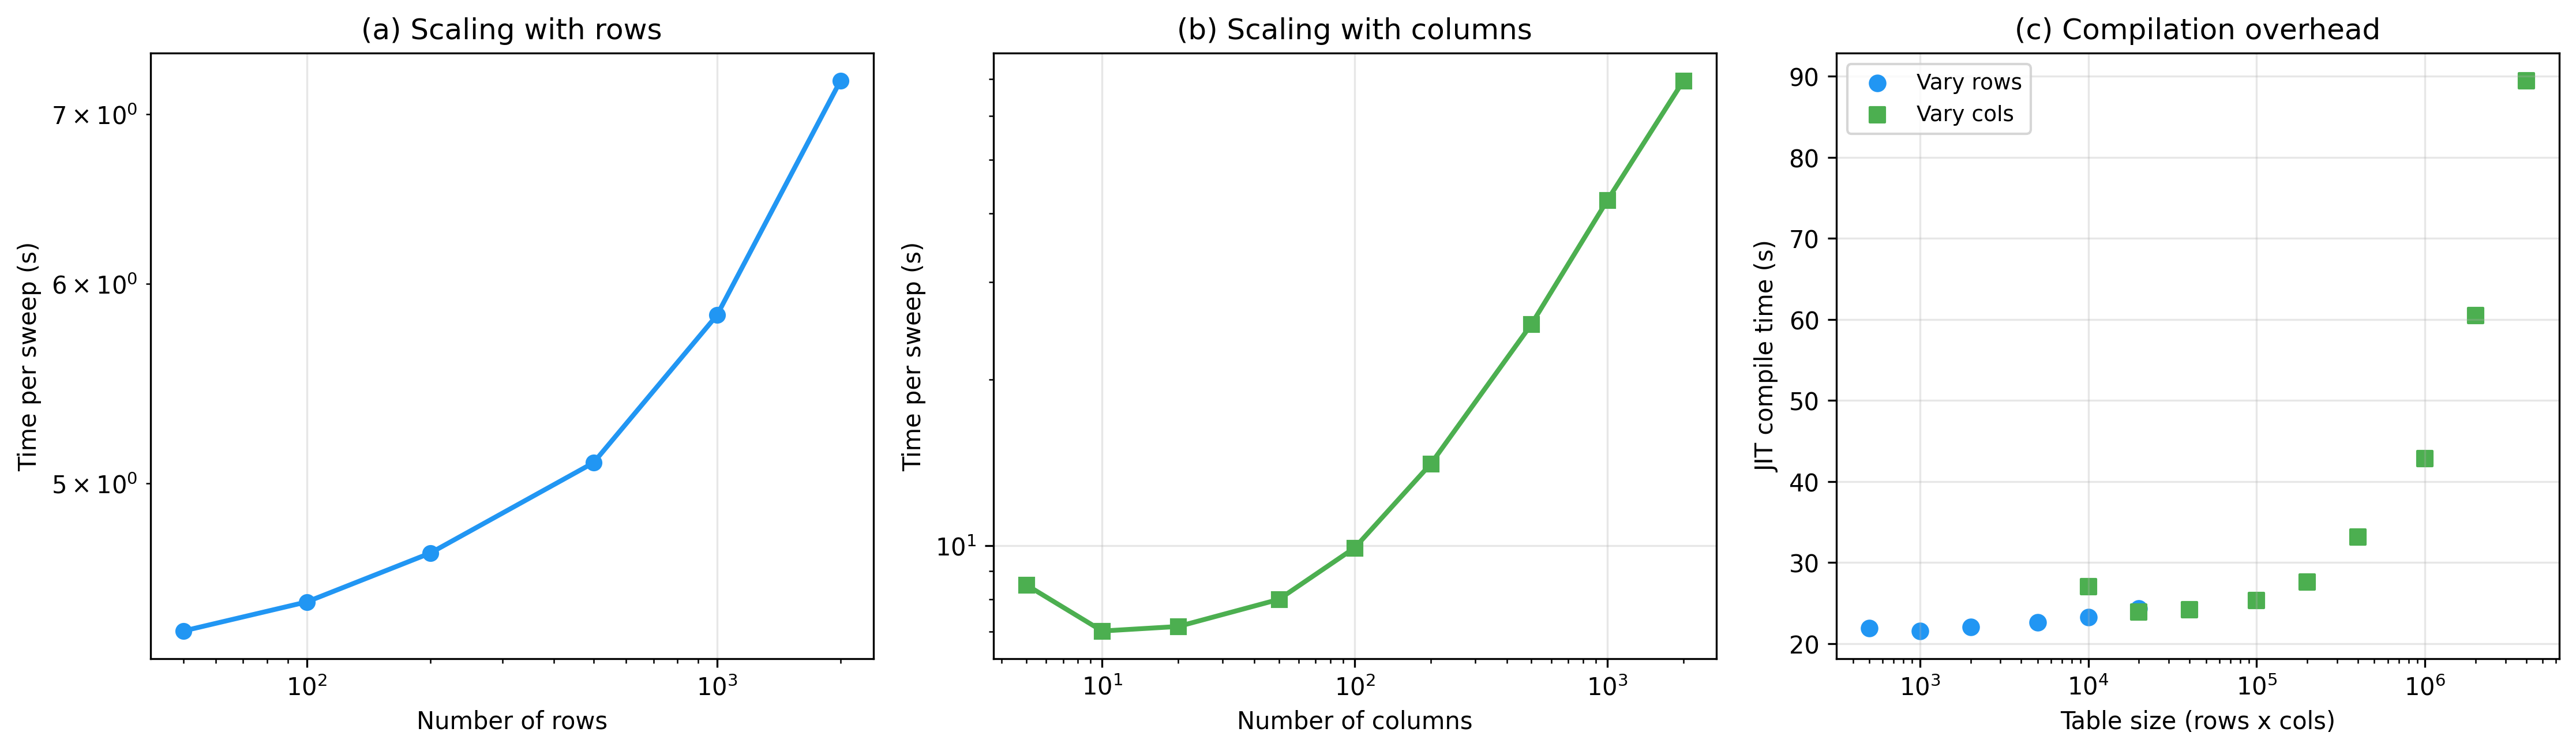
\includegraphics[width=0.95\textwidth]{figures/scalability.png}
\caption{Scalability of \jaxcc{} packed Gibbs sweep on $2\times$~T4 GPU.
  (a)~Per-sweep time vs.\ number of rows (10~cols).
  (b)~Per-sweep time vs.\ number of columns (2,000~rows).
  (c)~JIT compilation time vs.\ table size.}
\label{fig:scalability}
\end{figure}

\begin{table}[!htb]
\centering
\caption{Per-sweep wall-clock time on $2\times$~T4 GPU.}
\label{tab:scalability}
\begin{tabular}{rrrr}
\toprule
Rows & Cols & Compile (s) & Per sweep (s) \\
\midrule
50   & 10 & 21.9 & 4.37 \\
100  & 10 & 21.6 & 4.49 \\
200  & 10 & 22.1 & 4.69 \\
500  & 10 & 22.6 & 5.10 \\
1,000 & 10 & 23.3 & 5.83 \\
2,000 & 10 & 24.4 & 7.22 \\
\midrule
2,000 & 5   & 27.1 & 8.50 \\
2,000 & 10  & 23.9 & 7.02 \\
2,000 & 20  & 24.2 & 7.15 \\
2,000 & 50  & 25.3 & 8.00 \\
2,000 & 100 & 27.6 & 9.93 \\
2,000 & 200 & 33.2 & 14.08 \\
2,000 & 500 & 42.8 & 25.18 \\
2,000 & 1,000 & 60.5 & 42.22 \\
2,000 & 2,000 & 89.5 & 69.47 \\
\bottomrule
\end{tabular}
\end{table}

\paragraph{JIT compilation cost.} First compilation takes
${\sim}$22~seconds on T4 for a $200 \times 10$ problem, growing to
${\sim}$90~seconds for $2{,}000 \times 2{,}000$.
Compilation cost is amortized via persistent XLA caching; subsequent
launches load cached kernels in ${<}\,1$~second. Additionally,
per-sweep overhead decreases dramatically with batching: at 100~sweeps
per call, the amortized per-sweep time drops to 0.51~seconds (vs.\
23.3~seconds for a single sweep), as XLA dispatch overhead is paid once.

\paragraph{Multi-GPU throughput.} Using \texttt{jax.pmap} to distribute
4~chains across 2~T4 GPUs (2~chains per device), total wall-clock time
drops from 113.6s (sequential) to 34.7s, a $3.3\times$ speedup. The
speedup exceeds the theoretical $2\times$ because the sequential baseline
incurs per-chain dispatch overhead (compilation cache lookup, host-device
transfers) that pmap amortizes across all chains in a single launch.

\paragraph{Comparison to original.} The original
\texttt{probcomp/crosscat} implementation requires Python~2 and cannot be
run on modern systems for a direct wall-clock comparison. The kernel-level
benchmark (Table~\ref{tab:kernel_speedup}) compares the unpacked
(pure-Python) path to the packed path within \jaxcc{} itself on a P100
GPU. Individual kernels show $489$--$22{,}494\times$ speedups, with an
aggregate $619\times$ improvement. The full sweep achieves a lower
$43.6\times$ speedup because it additionally includes the column
assignment kernel (which requires sequential \texttt{lax.scan} over views
and is harder to parallelize) and because \texttt{packed\_gibbs\_sweep}
wraps all four kernels in a monolithic \texttt{lax.scan} whose XLA
compilation produces a larger, less-optimized trace compared to
individually JIT-compiled sub-kernels.

\begin{table}[!htb]
\centering
\caption{Kernel-level speedups: unpacked (Python loops) vs.\ packed
  (JIT+GPU) on a $200 \times 10$ dataset with 5 column types (P100 GPU).}
\label{tab:kernel_speedup}
\begin{tabular}{lrrr}
\toprule
Kernel & Unpacked (s) & Packed (s) & Speedup \\
\midrule
Row assignments    & 239.12 & 0.489 & 489$\times$ \\
Column hypers      & 65.35  & 0.003 & 22,494$\times$ \\
CRP alphas         & 0.59   & 0.001 & 946$\times$ \\
\midrule
Total (kernels)    & 305.05 & 0.493 & 619$\times$ \\
Full sweep (3 iter) & 994.21 & 22.82 & 43.6$\times$ \\
\bottomrule
\end{tabular}
\end{table}

% ============================================================================
\section{Software Engineering}
\label{sec:software}

\jaxcc{} comprises ${\sim}$12,500 lines of Python organized into
19~modules (Table~\ref{tab:modules}), excluding \texttt{\_\_init\_\_.py}
files. The packed sub-package (5~modules) contains the JIT-compiled
core; the remaining 14~modules provide initialization, unpacked
inference, diagnostics, serialization, scaling, and data utilities.

\begin{table}[!htb]
\centering
\small
\caption{Module organization of \jaxcc{}.}
\label{tab:modules}
\begin{tabular}{llp{6.5cm}}
\toprule
Module & Path & Purpose \\
\midrule
\texttt{types} & \texttt{crosscat/} & State dataclasses, column type enum \\
\texttt{components} & \texttt{crosscat/} & Conjugate Bayesian component models \\
\texttt{model} & \texttt{crosscat/} & Initialization, log joint, row insertion \\
\texttt{gibbs} & \texttt{crosscat/} & Unpacked Gibbs kernels (reference) \\
\texttt{inference} & \texttt{crosscat/} & Unpacked inference queries \\
\texttt{packed\_inference} & \texttt{crosscat/} & Vectorized packed inference queries \\
\midrule
\texttt{packed/state} & \texttt{packed/} & Packed state, pack/unpack, batching \\
\texttt{packed/components} & \texttt{packed/} & Unified type dispatch, batch scoring \\
\texttt{packed/suffstats} & \texttt{packed/} & Vectorized sufficient statistics \\
\texttt{packed/kernels} & \texttt{packed/} & JIT-compiled Gibbs kernels \\
\texttt{packed/aot\_cache} & \texttt{packed/} & XLA persistent compilation cache \\
\midrule
\texttt{constraints} & \texttt{crosscat/} & Column/row dependency constraints \\
\texttt{diagnostics} & \texttt{crosscat/} & Convergence metrics (ARI, log-lik) \\
\texttt{serialization} & \texttt{crosscat/} & Save/load in \texttt{.jxc} format \\
\texttt{synthetic} & \texttt{crosscat/} & Synthetic data generation \\
\texttt{data\_utils} & \texttt{crosscat/} & CSV I/O, type detection \\
\texttt{scaling} & \texttt{crosscat/} & Subsample init, mini-batch Gibbs, early stop \\
\texttt{tb\_logger} & \texttt{crosscat/} & TensorBoard diagnostics logging \\
\texttt{validate} & \texttt{crosscat/} & State consistency checking \\
\bottomrule
\end{tabular}
\end{table}

\paragraph{Testing.} The test suite includes 333~tests: 289~fast tests
(including 34~Hypothesis property tests verifying mathematical invariants
such as sufficient statistic roundtrips, component model scoring, type
dispatch parity, and NaN safety) and 44~slow GPU-intensive tests marked
with \texttt{@pytest.mark.slow}. Property tests ensure correctness
across all five column types for random inputs.

\paragraph{Serialization.} Model states are saved in \texttt{.jxc}
format (JSON metadata + NPZ arrays) with schema versioning (currently
v3) and backward migration support. Additional I/O formats include
memory-mapped NumPy (\texttt{.npy}) for multi-GB datasets and Apache
Parquet via \texttt{pyarrow}.

\paragraph{Installation.} \jaxcc{} requires Python~3.11+ and is
installable via \texttt{pip}. GPU support requires a CUDA-enabled JAX
backend.

% ============================================================================
\section{Related Work}
\label{sec:related}

\paragraph{Original CrossCat.} \citet{mansinghka2016crosscat} introduced
the model, inference algorithm, and extensive empirical evaluation. Our
work preserves full algorithmic fidelity while providing a modern,
GPU-accelerated implementation. A commercial implementation (Veritable,
later acquired by Salesforce) demonstrated scalability to million-row
datasets \citep{obermeyer2014scaling}, but is not publicly available.

\paragraph{BayesDB and Loom.} BayesDB \citep{mansinghka2015bayesdb}
provides a SQL-like interface to CrossCat via the \texttt{cgpm}
metamodeling framework. Loom \citep{loom} is a C++ implementation
focused on speed, using a ``kind'' representation similar to our packed
state. Loom can handle millions of rows on CPU via streaming
architecture and cache-friendly data structures; \jaxcc{} trades
maximum row count for GPU throughput on medium-sized tables
(${\sim}$200--2,000~rows) with many columns. Both are complementary:
Loom for large-$R$, small-$D$ workloads; \jaxcc{} for moderate-$R$,
large-$D$ workloads with rich inference queries.

\paragraph{JAX ecosystem.} JAX \citep{jax2018github} has enabled
GPU-accelerated reimplementations of classical probabilistic methods,
including NumPyro \citep{phan2019composable} for probabilistic
programming and BlackJAX \citep{cabezas2024blackjax} for MCMC kernels.
\jaxcc{} follows this trend for nonparametric mixture models.

\paragraph{Alternative nonparametric methods.} Hierarchical Dirichlet
processes \citep{teh2006hierarchical}, nested Dirichlet processes
\citep{rodriguez2008nested}, and variational alternatives
\citep{guan2010variational} address related modeling problems. CrossCat's
unique contribution is the column-wise DP that discovers independence
structure, which none of these alternatives provide.

% ============================================================================
\section{Discussion and Limitations}
\label{sec:discussion}

\paragraph{Practical limits.} The current benchmarks cover datasets up
to $2{,}000 \times 2{,}000$ cells, with scaling utilities (subsample
annealing, mini-batch Gibbs) designed for 10K--1M+ rows. The original
CrossCat paper reports results on tables of up to 10~million cells;
reaching this scale in \jaxcc{} is supported by the \texttt{scaling}
module but has not yet been validated end-to-end. For the MNIST
benchmark (\texttt{max\_views}${}=16$, \texttt{max\_clusters}${}=32$,
257~columns), the packed state consumes ${\sim}$25~MB per chain ---
modest on modern GPUs. Multi-GPU execution via \texttt{jax.pmap}
distributes chains across devices, achieving near-linear throughput
scaling ($3.3\times$ on 2~GPUs). However, the single-site row sweep
is inherently sequential ($O(R)$ per view), so per-chain throughput
scales linearly with rows. Mini-batch row transitions ($O(B)$ per
sweep) mitigate this for large datasets.

\paragraph{Limitations.} (1)~The packed representation wastes memory for
highly unbalanced states (many views with few columns or vice versa).
(2)~JIT compilation time grows to ${\sim}$90~seconds for
$2{,}000 \times 2{,}000$ problems, though persistent caching and
sweep batching (amortized cost 0.51~s/sweep at 100~sweeps) mitigate
this. (3)~The single-site Gibbs sampler can mix slowly for strongly
coupled structures; split-merge moves \citep{jain2004split} could
improve this. (4)~Within-component models assume conditional independence
between columns given the cluster; this limits the ability to capture
within-cluster correlations. (5)~Cross-indicator imputation on raw
scales (as in the WDI benchmark) yields moderate aggregate correlation
($r = 0.53$) due to scale heterogeneity, though per-indicator accuracy
is substantially higher.

\paragraph{Future work.} Planned extensions include: additional component
models (e.g., Poisson, zero-inflated); split-merge proposals for faster
mixing; end-to-end validation of scaling utilities at 100K--1M+ rows;
and integration with probabilistic programming frameworks.

% ============================================================================
\section{Conclusion}

We presented \jaxcc{}, a GPU-accelerated reimplementation of CrossCat in
JAX. By combining a packed state representation, unified type dispatch,
vectorized Gibbs kernels, batched sufficient statistics, and multi-GPU
execution via \texttt{jax.pmap}, \jaxcc{} brings the full power of
CrossCat's nonparametric Bayesian analysis to modern GPU hardware. We
reproduced the key experiments from the original paper, demonstrated
scalability up to $2{,}000 \times 2{,}000$ tables, and introduced scaling
utilities for datasets with 10K+ rows. The library provides 29
vectorized inference queries, 333~tests, and is available at
\url{https://github.com/sambhal-labs/jaxcross}.

% ============================================================================
\section*{Acknowledgments}

We acknowledge \citet{mansinghka2016crosscat} for the CrossCat model and
inference algorithm upon which this work builds. GPU resources were
provided by Kaggle and Google Colab.

% ============================================================================
\bibliographystyle{plainnat}
\bibliography{references}

% ============================================================================
\appendix

\section{Inference Query Reference}
\label{app:queries}

Table~\ref{tab:queries} lists all packed inference queries provided by
\jaxcc{}.

\begin{table}[!htb]
\centering
\small
\caption{Packed inference queries in \jaxcc{}.}
\label{tab:queries}
\begin{tabular}{lp{7cm}}
\toprule
Function & Description \\
\midrule
\texttt{packed\_predictive\_probability} & Log-probability of a value given context \\
\texttt{packed\_predictive\_sample} & Sample from posterior predictive \\
\texttt{packed\_predictive\_cdf} & Empirical CDF via MC sampling \\
\texttt{packed\_anomaly\_score} & Row anomalousness via avg.\ log-prob \\
\texttt{packed\_impute\_and\_confidence} & Point estimate + confidence \\
\texttt{packed\_credible\_interval} & Percentile-based intervals \\
\texttt{packed\_mutual\_information} & MC estimate of mutual information \\
\texttt{packed\_dependence\_probability} & View co-assignment probability \\
\texttt{packed\_dependence\_matrix} & Full Z-matrix (pairwise) \\
\texttt{packed\_row\_similarity} & Category co-assignment probability \\
\texttt{packed\_row\_typicality} & Typicality under model \\
\texttt{packed\_column\_typicality} & Column typicality \\
\texttt{packed\_conditional\_entropy} & Conditional entropy estimate \\
\texttt{packed\_joint\_predictive\_probability} & Joint log-probability \\
\texttt{packed\_sample\_and\_insert} & Sample new row and insert \\
\midrule
\multicolumn{2}{l}{\textit{Batch-vectorized variants (vmapped over rows/columns):}} \\
\texttt{batch\_classify\_column} & Classify all rows for a target column \\
\texttt{batch\_score\_columns\_binary} & $P(\text{col}=1)$ for multiple binary columns \\
\texttt{batch\_anomaly\_score} & Anomaly scores for all rows \\
\texttt{batch\_impute\_column} & Impute a column for multiple rows \\
\texttt{batch\_row\_similarity} & Pairwise row similarity matrix \\
\texttt{batch\_row\_typicality} & Typicality for multiple rows \\
\texttt{batch\_predictive\_cdf} & CDF for multiple rows \\
\texttt{batch\_credible\_interval} & Credible intervals for multiple rows \\
\midrule
\multicolumn{2}{l}{\textit{Multi-chain wrappers (aggregate across chains):}} \\
\texttt{multi\_chain\_predictive\_probability} & Averaged log-prob across chains \\
\texttt{multi\_chain\_predictive\_sample} & Sample from chain mixture \\
\texttt{multi\_chain\_anomaly\_score} & Averaged anomaly across chains \\
\texttt{multi\_chain\_impute\_and\_confidence} & Averaged imputation \\
\texttt{multi\_chain\_predictive\_cdf} & Averaged CDF across chains \\
\bottomrule
\end{tabular}
\end{table}

\end{document}
